\documentclass{elteikthesis}

\usepackage{url}
\usepackage{fancyhdr}
\usepackage{indentfirst}
\usepackage{enumitem}
\usepackage{ucs}
\usepackage{xcolor}
\usepackage{float}
\usepackage[utf8]{inputenc}
\usepackage[nottoc,numbib]{tocbibind}
\usepackage[T1]{fontenc}
\usepackage[english,hungarian]{babel}
\selectlanguage{hungarian}

\title{Rendezési algoritmusok szemléltetése}
\author{Márföldi Péter Bence}
\supervisor{Veszprémi Anna}
\supervisorstitle{mestertanár}
\period{programtervező informatikus BSc}
\thesisyear{2015}
\department{Algoritmusok és Alkalmazásaik Tanszék}

\fancyhf{}
\fancyhead[L]{\rightmark}
\fancyfoot[C]{\thepage}
\definecolor{default}{HTML}{F3622D}
\definecolor{swap}{HTML}{4258C9}
\definecolor{select}{HTML}{57B757}
\definecolor{done}{HTML}{8C2D46}

\begin{document}

\frontmatter

	\maketitle
	\renewcommand{\thepage}{\Roman{page}}
	\tableofcontents\thispagestyle{fancy}
	
\mainmatter
	\pagestyle{fancy}
	\setlist[description]{leftmargin=\parindent,labelindent=\parindent,itemsep=1.5pt}

\chapter{Bevezetés} 
 Az eddigi egyetemen töltött éveim során az \textbf{Algoritmusok és adatszerkezetek} kurzus foglalkozott mélyrehatóan a rendezési algoritmusokkal. Számomra a tananyagból talán ez a témakör volt a legnehezebben elsajátítható. Ez sarkallt arra, hogy a szakdolgozatom témáját adják a rendezési algoritmusok, szerettem volna biztos tudással rendelkezni ezen a területen.\par
 Az bizonyos, hogy minden informatikus - beleértve a leendőeket is - tanulmányaik kezdetén találkoztak a rendezési algoritmusokkal. Nagyszerű terület arra, hogy megérthessük mi egy algoritmus műveletigénye, hogy mi számít igazán sok adatnak, vagy, hogy mit értünk egy algoritmus stabilitásán.\par

\section{A feladat és annak értelmezése} 

\section{Alkalmazott technológiák}
A Következőkben röviden összefoglaljuk a \emph{Java}\cite{Java}, \emph{JavaFX}\cite{JavaFX} és \emph{JUnit}\cite{JUnit} jellegzetességeit.
\subsection{Java}
A \emph{Java} egy általános célú, objektumorientált programozási nyelv, melyet 2009-ig a \emph{Sun Microsystems} fejlesztett, ezt követően pedig az \emph{Oracle}. A szakdolgozatban használt 1.8-as verziót már az \emph{Oracle} adta ki 2014-ben. A \emph{Java} nyelv a szintaxisát a \emph{C} és \emph{C++} nyelvektől örökölte, azonban utóbbitól eltérően egyszerű objektummodellel rendelkezik. \par
 A \emph{Java} platformra készült programok túlnyomó többsége asztali alkalmazás. Manapság egyre több helyen találkozhatunk a \emph{Java} nyelven írt programokkal, például mobil eszközökön, banki rendszereknél vagy akár egy szórakoztató elektronikai eszközön. Nagy előnye, hogy sok nyelvvel ellentétben platformfüggetlen, azaz egy adott platformról egy program minimális változtatással átültethető egy másik platformra. \par
 A \emph{Java} legfontosabb része a \emph{Java virtuális gép (JVM)}. A \emph{JVM}-et sokféle berendezés és szoftvercsomag tartalmazza, így a nyelv egyaránt platformként és középszintként is működik.
Összefoglalva a \emph{Java} program három fontos szerepet tölt be:
\begin{description}
\item[$\bullet$] programozási nyelv
\item[$\bullet$] köztes réteg (middleware)
\item[$\bullet$] platform
\end{description}

\subsection{JavaFX}
Olyan szoftverplatform, amelynek célja, hogy gazdag internetes alkalmazást lehessen készíteni és futtatni eszközök széles skáláján. Eredetileg a \emph{Swing} könyvtárat váltotta volna fel, azonban jelenleg mindkettő része a \emph{Jave SE}-nek. \par
 A 2.0-ás verzióig a fejlesztők egy külön nyelvet használtak, amelyet \emph{JavaFX Script}-nek neveznek. Azonban mivel ez szintén \emph{Java} bájtkódot generál a későbbiekben megadatott a lehetőség, hogy a programozók Java kódot használjanak helyette. A \emph{JavaFX} egyik legnagyobb előnye, hogy egy egyszerű \emph{XML} struktúrában leírhatók a program grafikus felületének összetevői, melyhez ezt követően elegendő az egyes interakciókhoz tartozó funkciókat implementálni.\par Az elterjedtebb operációs rendszerek mindegyikét támogatja. Ahogyan előnye, úgy hátránya is a \emph{Swing}-hez képest az, hogy jelenleg is folyik a fejlesztése, ezért olykor csak hosszas utánajárást követően sikerül megoldást találni egy-egy problémára.
 
\subsection{JUnit}
Egy egységteszt keretrendszer a \emph{Java} programozási nyelvhez. Az egységtesztek karbantartására, és futtatására kínál szolgáltatást. Gyakran a verzió kiadási folyamat részeként szokták beépíteni, azaz egy kiadás akkor hibátlan, ha ezen tesztek mindegyike hibátlanul lefut. Egy 2013-as felmérésben\cite{Survey} tízezer Java technológiát használó \emph{GitHub} projektet vizsgáltak. A projektek csaknem harmadánál használták a \emph{JUnit}-ot, ezzel az egyik leggyakrabban használt függvénykönyvtár volt a felmérés során.

\chapter{Felhasználói dokumentáció}
\section{Rendszerkövetelmények}
Az elkövetkezőkben ismertetésre kerülnek a minimális és az ajánlott rendszerkövetelmények.
\subsection{Minimális rendszerkövetelmények}
Mivel a program \emph{Java} nyelven íródott, ezért elengedhetetlen, hogy a felhasználó számítógépén lehetőség legyen \emph{Java} alkalmazások futtatására. Az alábbi operációs rendszereken érhető el a \emph{Java Runtime Enviroment 8u45}-ös verziója:\par
\begin{description}
	\item[$\bullet$] \emph{Windows} 8
	\item[$\bullet$] \emph{Windows} 7
	\item[$\bullet$] \emph{Windows} Vista SP2
	\item[$\bullet$] \emph{Windows Server} 2008 R2 SP1 (64-bit)
	\item[$\bullet$] \emph{Windows Server} 2012 (64-bit)
	\item[$\bullet$] \emph{Mac OS X} 10.8.3 vagy újabb
	\item[$\bullet$] \emph{Suse Linux Enterprise Server} 10 SP2+, 11.x
	\item[$\bullet$] \emph{Ubuntu Linux} 12.04 vagy újabb
	\item[$\bullet$] \emph{Red Hat Enterprise Linux} 5.5+, 6.x
	\item[$\bullet$] \emph{Oracle Linux} 5.5+; 6.x; 7.x
\end{description}
Hardverkövetelmények tekintetében a \emph{Java JRE 8} futtatásához szükséges
minimum követelményei az irányadóak. Azonban a program bizonyos esetekben több erőforrást is igényelhet, ezért ajánlott nagyobb memóriával és erősebb processzor rendelkező rendszer használata. A követelmények a következő táblázatban találhatóak:\par
\begin{table}[h]
		\def\arraystretch{2}
		\centering
	\begin{tabular}{|l|l|}
		\hline
		\textbf{Memória}           & 128 MB            \\ \hline
		\textbf{Szabad lemezterület} & 124 (+2) MB       \\ \hline
		\textbf{Processzor}          & \emph{Pentium} 2 266 MHz \\ \hline
	\end{tabular}
\end{table}
\subsection{Ajánlott rendszerkövetelmények}
A szoftver tökéletes működéséhez a legelterjedtebb operációs rendszer, a \emph{Windows} ajánlott. Továbbá követelmény 16:9-es képaránnyal rendelkező monitor, és legalább 1366$\times$768 képernyőfelbontás használata.\par
A rendszer fejlesztése a következő ajánlott konfiguráción történt:
\begin{table}[h]
	\def\arraystretch{2}
	\centering
	\begin{tabular}{|l|l|}
		\hline
		\textbf{Operációs rendszer} & \emph{Windows} 7                     \\ \hline
		\textbf{Memória}            & 4 GB                          \\ \hline
		\textbf{Processzor}         & \emph{Intel} Core i5-2467M, 2000 MHz \\ \hline
	\end{tabular}
\end{table}

\subsection{Telepítés és eltávolítás}
Alapvetően elegendő a \emph{Java} futtatási környezet telepítéséről gondoskodnia a felhasználónak, ezen felül más program telepítésére nincs szükség. Azonban, mivel elsősorban \emph{Windows} operációs rendszeren történő futtatásra lett felkészítve a program, ezt az operációs rendszert használók választhatják a kényelmesebb, natív telepítéses megoldást. Elsőként a programhoz készült telepítővel történő konfigurálást vesszük végig, majd ezt követően a \emph{Java} programokra inkább jellemzőbb, ám kissé körülményesebb telepítési mód kerül bemutatásra. Végül röviden összefoglaljuk a program eltávolításához szükséges lépéseket.
\par Bármely módszert is szándékozik követni a felhasználó, először győződjön meg róla, hogy az előzőekben ismertetett rendszerkövetelményeknek megfelel a számítógépe

\subsubsection{Telepítés natív telepítővel}
Ez a telepítési mód csak a \emph{Windows}-t használók számára érhető el.\par
Az első lépés a telepítési varázsló elindítása. A megjelenő párbeszédpanelon kattintsunk a \textbf{Telepítés} gombra. Ezt követően elindul a telepítés, ami körülbelül fél percet vesz igénybe.\par
\begin{figure}[H]
	\centering
	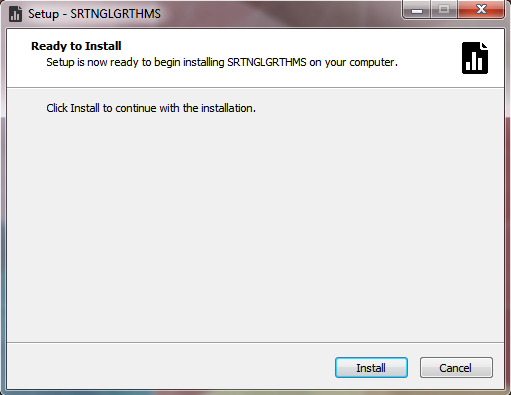
\includegraphics[width=0.6\textwidth]{pics/setup.png}
	\caption{A telepítési párbeszédpanel}
\end{figure}\par
A telepítési panel bezárása után máris megjelenik a program főmenüje, így megkezdheti a felhasználó a használatát. A későbbiekben történő futtatáshoz a következő könyvtárba szükséges navigálni: \textbf{C:\textbackslash Felhasználók\textbackslash \{Felhasználói név\}\textbackslash AppData\textbackslash Local\textbackslash SRTNGLGRTHMS\textbackslash SRTNGLGRTHMS.exe} \par
A fenti útvonal akkor érvényes, ha \textbf{C:\textbackslash} meghajtón található az operációs rendszer, néhány rendszeren más lehet ennek a meghajtónak a betűjele. Továbbá egyes számítógépeken az \textbf{AppData} mappa rejtett lehet, így érdemes valamilyen fájlböngészőt, például \emph{Total Commander}-t használni.

\subsubsection{Hagyományos telepítés}
A most ismertetésre kerülő telepítési mód minden operációs rendszeren elérhető.\par
Az első feladat a \emph{Java} virtuális gép telepítése, amely letölthető a következő webcímről: \url{http://java.com/inc/BrowserRedirect1.jsp}\par
Fogadjuk el a licencszerződést, töltsük le a \emph{JRE} telepítőfájlt. Ha frissíteni szeretnénk a jelenlegi \emph{Java} verziót a rendszerünkön, akkor előbb célszerűbb eltávolítani a régi verziót. Miután feltelepítettük a futtatási környezetet,  készen áll a szoftver futtatására a rendszerünk. A program könyvtárában található \textbf{SRTNGLGRTHMS.jar} fájl elindításával kezdhetjük meg a szoftver használatát.

\subsubsection{Eltávolítás}
A program törlése az utóbb ismertetett telepítési mód esetében mindössze annyiból áll, hogy a \textbf{SRTNGLGRTHMS.jar} fájlt eltávolítjuk, valamint amennyiben a jövőben nincs igény a \emph{Java} futtatási környezet használatára, úgy a felhasználó eltávolíthatja azt.
\emph{Windows}-on történő natív telepítést követően a program telepítési könyvtárában található \textbf{unins000.exe} fájlt futtatva, majd az \textbf{Igen} gombra kattintva a program törlődik a számítógépről.

\section{Felhasználói felület bemutatása}
\subsection{Főmenü}
A program indítását követően megjelenik a főmenü, mely két komponensből áll.\par
\begin{figure}[H]
	\centering
	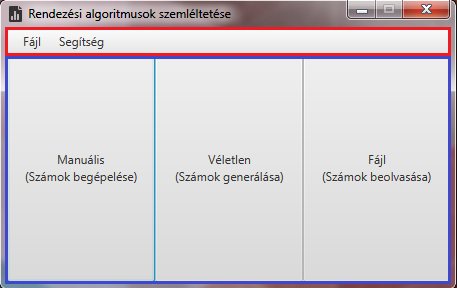
\includegraphics[width=0.7\textwidth]{pics/mainmenu.png}
	\caption{A program főmenüje}
\end{figure}\par
  Az ablak felső részén található piros színnel jelölt rész az eszköztárat foglalja magában. A kék szín jelöli a főmenü központi paneljét, mely három gombból tevődik össze. Ezen gombokra történő kattintás után lehetőség nyílik a rendezendő számok megadására.

\subsubsection{Eszköztár}
Az eszköztárat két menüpont alkotja, \textbf{Fájl} és \textbf{Segítség} címszóval ellátva. Az előzőben a program bezárásának lehetősége kapott helyet, míg utóbbiban a szoftver névjegye tekinthető meg. Az \textbf{Ok} gomb lenyomásával bezárható a névjegy.
\begin{figure}[H]
	\centering
	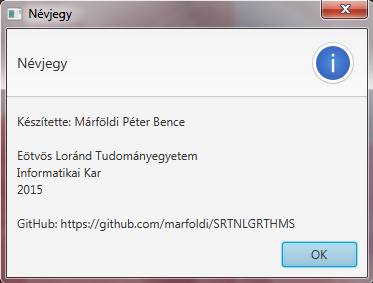
\includegraphics[width=0.5\textwidth]{pics/about.png}
	\caption{A program névjegye}
\end{figure}\par

\subsubsection{Központi panel}
A három gombból áll:
\begin{description}
	\item[$\bullet$] Manuális (számok begépelése)
	\item[$\bullet$] Generálás (számok generálása) 
	\item[$\bullet$] Fájl (számok beolvasása)
\end{description}
Ezek közül bármelyre kattintva átnavigálhatunk a bement megadását lehetővé tévő felületekre.

\subsection{Bemenet megadása panel}
Az előzőekben említett három lehetőség közül választhat a felhasználó.

\subsubsection{Manuális}
A megjelenő panelen két gomb található, melyek kezdetben inaktívak. A "Méret:" címke után található beviteli mezőbe egy pozitív egész szám megadásával és az \textbf{ENTER} billentyű leütésével megjelennek a számok bevitelére lehetőséget adó mezők. Ezt követően a panelen található két gomb már kattintható, a \textbf{Számok generálása} gombra kattintva 0 és 100 közötti véletlen számokkal töltődnek fel a mezők. Az \textbf{Ok}ra történő kattintás után megjelenik a program \textbf{Főpanel}je.\par
\begin{figure}[H]
	\centering
	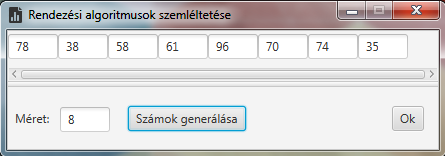
\includegraphics[width=0.6\textwidth]{pics/manualinput.png}
	\caption{8 elemű manuálisan megadott bemenet}
\end{figure}
Meg kell jegyezni, hogy ebben a módban legfeljebb száz érték adható meg, ennél nagyobb méretű bemenet manuális feltöltése túl körülményes lenne. Amennyiben több számot szándékozik megadni a felhasználó, válasszon a számok generálása vagy a fájlból történő beolvasás lehetőségek közül.

\subsubsection{Generálás}
A "Méret:" címke mellett megadva a bemeneti számok mennyiségét, és a legördülő menüből kiválasztva a generálás módját az \textbf{OK} gomb kattinthatóvá válik.
\begin{figure}[H]
	\centering
	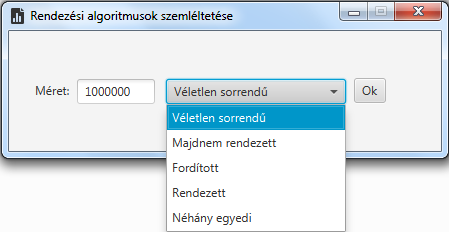
\includegraphics[width=0.6\textwidth]{pics/randominput.png}
	\caption{Egymillió véletlen generált érték megadása}
\end{figure}
 A legördülő menüből a következő négy típus közül lehet választani, azaz a generált tömb legyen:
\begin{description}
	\item[$\bullet$] Véletlen generált - véletlenszerűen választott számokból álljon
	\item[$\bullet$] Majdnem rendezett - a tömb 80\%-a már rendezve legyen
	\item[$\bullet$] Fordított - a tömb legyen csökkenőleg rendezett
	\item[$\bullet$] Néhány egyedi - a tömb elemei között sok azonos érték szerepeljen
\end{description}
Itt megjegyzendő, hogy amennyiben az input mérete az [1,100] intervallumban van, akkor a rendezendő számok a 0 és 100 közötti értékek közül kerülnek kiválasztásra. Ennek oka, hogy a túl nagy differencia az egyes értékek között sokat rontana az oszlopdiagramok megjelenésén. Ellenkező esetben a \emph{Java} nyelv által definiált egész típus(\emph{Integer}) maximális értékéig terjedhet a generált számok nagysága.
 
\subsubsection{Fájl - fájlból beolvasás}
A gombra történő kattintás után megjelenik egy fájltallózó. A tallózóban csak szöveges(\emph{txt} kiterjesztésű) fájl választására van lehetőség.
\begin{figure}[H]
	\centering
	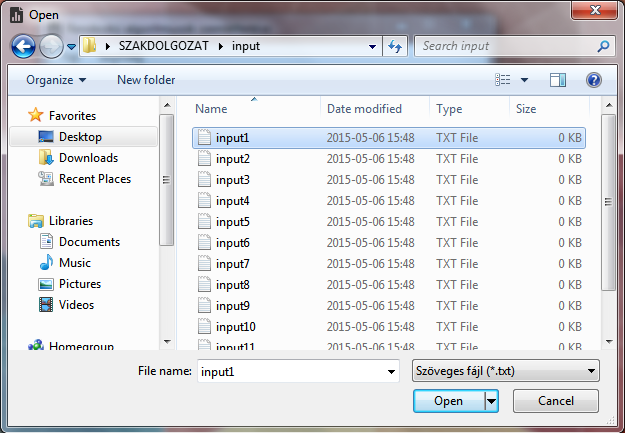
\includegraphics[width=0.6\textwidth]{pics/fileinput.png}
	\caption{Fájltallózó}
\end{figure}
 A fájl tartalmára történő megszorítások szigorúak. Minden sora legfeljebb egy pozitív egész számot tartalmazhat, ellenkező esetben a program hibaüzenet kíséretében visszatér a főmenübe. Fontos, hogy az előzőek értelmében az üres sorok sem megengedettek.
 \begin{figure}[H]
 	\centering
 	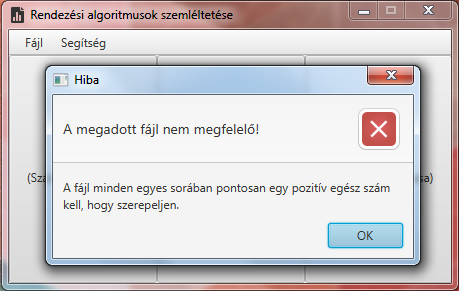
\includegraphics[width=0.6\textwidth]{pics/fileinput_error.png}
 	\caption{Nem megfelelő fájl esetén a hibaüzenet}
 \end{figure}

\subsection{Főpanel}
A rendezendő számok sikeres megadása után megjelenik a program főpanelje, mely három logikai részből áll. A főpanel magában foglalja a \textbf{Megfigyelés} és \textbf{Összehasonlítás} paneleket, melyek összetettségükből fakadóan külön alfejezetekben kerülnek részletezésre.
 \begin{figure}[H]
 	\centering
 	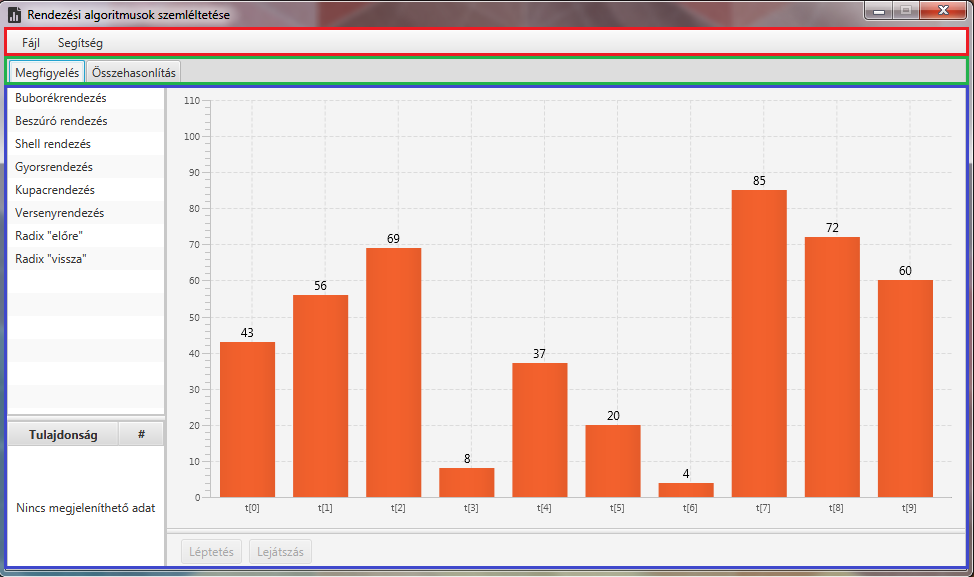
\includegraphics[width=0.8\textwidth]{pics/mainpanel.png}
 	\caption{A program főpanelja}
 \end{figure}
\subsubsection{Eszköztár}
A \textbf{Főmenü}höz hasonlóan itt is jelen van a piros színnel jelzett eszköztár sáv. Itt fontos kiemelni, hogy a \textbf{Fájl} és \textbf{Segítség} pontokon belül további alpontok is elérhetőek:\par
A \textbf{Fájl} menüpont bővül a \textbf{Vissza a főmenübe} lehetőséggel, melynek segítségével a program újraindítása nélkül lehetőség van újabb rendezendő számsorozat megadására.\par
A \textbf{Segítség}re kattintva további lehetőségként választható az \textbf{Algoritmusról} pont. Itt elolvasható a rövid szöveges ismertetője a \textbf{Megfigyelés} panel listájából kiválasztott elemnek. Amennyiben pedig az \textbf{Összehasonlítás} panel aktív, akkor e panel táblázatából kiválasztott algoritmus leírása tekinthető meg. Az aktuális panelen ha nem került kiválasztásra sor, akkor a menüpontra történő kattintás után felugró ablak figyelmezteti a felhasználót arról, hogy e menüpont használatához előbb ki kell választani egy algoritmust.
\subsubsection{Panelválasztó}
Amennyiben a bemenet megadásánál már ismertetett [1,100] intervallum magában foglalja a bemenet hosszát, akkor két elem látható a zöld jelölt részen. Így lehetősége van a felhasználónak navigálni a \textbf{Megfigyelés} és az \textbf{Összehasonlítás} panel között. Ellenkező esetben csak az utóbbi panel jelenik meg. Az aktuálisan megjelenített felület neve a listában kék kerettel jelenik meg, valamint a másik elemhez képest világosabb szürke színnel.
\subsubsection{Panel}
A harmadik logikai egységet alkotják a panelek - kék színnel jelölve -, melyek közötti váltást a \textbf{Panelválasztó} teszi lehetővé. Mivel részletesebb leírást kíván a panelek ismertetése, ezért egy-egy külön alfejezetben kerülnek bemutatásra.

\subsection{Megfigyelés panel}
A főpanel középső területén foglal helyet, négy komponensből tevődik össze. A felhasználónak itt nyílik lehetősége az egyes algoritmusok megfigyelésére, tanulmányozására.
 \begin{figure}[H]
 	\centering
 	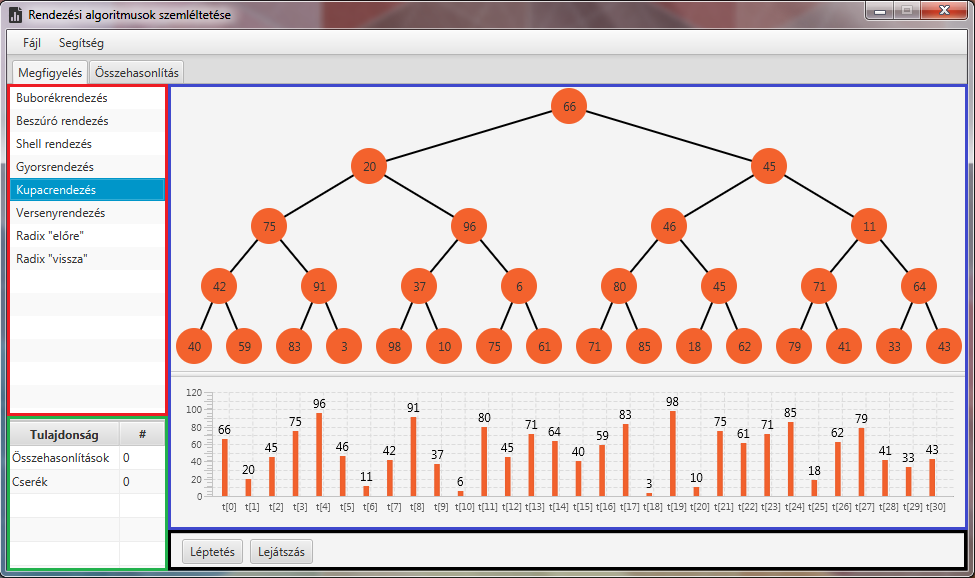
\includegraphics[width=0.8\textwidth]{pics/watchpanel.png}
 	\caption{Megfigyelés panel}
 \end{figure}
\subsubsection{Algoritmus lista}
Az ábrán piros színnel jelölt rész, melynek elemeire kattintva kiválasztható, hogy mely algoritmust szeretné a felhasználó vizsgálni. A kiválasztott elem kék háttérszínt kap, alapértelmezett esetben nincs kijelölt elem.
\subsubsection{Állapotjelző táblázat}
A kiválasztott algoritmus aktuális állapotához tartozó információk jelennek meg a táblázatban. Az ábrán zöld kerettel van jelölve a komponens. Amennyiben nincs kiválasztott elem a \textbf{Nincs megjeleníthető adat} szöveg jelenik meg.\par
Két oszlopa a \textbf{Tulajdonság} és a \textbf{\#}, mely utóbbi az értéket jelöli. Alapvetően az összehasonlításon alapuló algoritmusoknál megjelenő adatok az összehasonlítások és cserék vagy mozgatások száma. Az edényrendezéseknél pedig az aktuálisan vizsgált bit indexe és a vizsgálatok száma jelenik meg. Egyes algoritmusokhoz a jobb megérhetőség miatt további állapotjelző értékek is tartoznak, melyek a következők:
\begin{table}[h]
	\centering
	\begin{tabular}{|c|c|}
		\hline
		\textbf{Algoritmus} & \textbf{Tulajdonság} \\ \hline
		Shell rendezés      & Lépésköz             \\ \hline
		Gyorsrendezés       & Vezérelem            \\ \hline
		Radix "előre"       & Cserék száma         \\ \hline
	\end{tabular}
\end{table}
\subsubsection{Gombok}
Alaphelyzetben a \textbf{Léptetés} és \textbf{Lejátszás} gombok inaktívak. A képen fekete keretet jelzi a helyüket. Amennyiben a felhasználó kiválaszt egy elemet az algoritmus listáról kattinthatóvá vállnak. A léptetéssel egy következő állapotot tekinthet meg a felhasználó. A \textbf{Lejátszás} gombra kattintva a program bemutatja az algoritmus működését. A felhasználó bármikor megállíthatja az animációt a \textbf{Lejátszás} gomb helyén található \textbf{Megállítás} gombra kattintva, majd ha kívánja innen folytathatja a vizsgálatot. Amennyiben a rendezés lezajlott, megjelenik az \textbf{Újraindítás} gomb, melynek megnyomásával az értékek visszakerülnek az eredeti helyükre.

\subsubsection{Állapotjelző felület}
A fenti ábrán kék szín jelöli ezt a területet.
Az állapotjelző felületen minden esetben legalább egy oszlopdiagram foglal helyet. Ettől eltérően a \textbf{Kupac}- és \textbf{Versenyrendezés} kiválasztásakor egy gráf is helyet kap. Továbbá a \textbf{Radix "vissza"} rendezés második tömbjének reprezentálásához egy plusz oszlopdiagram is megjelenik. Itt megjegyzendő, hogy a szemléltetéshez használt bináris fa legfeljebb 31 csúcsot tartalmazhat. Hosszabb bemenet megadásakor csak az első 31 elem vesz részt a megjelenítésben.
\par Az egyes műveleteket különböző színek is jelölik. Alapértelmezetten a rendezendő elemek színe a következőket jelentik:\par
\begin{description}
	\item[\textcolor{default}{\Huge$\bullet$}] Az alapértelmezett szín, nincs kijelölve az elem.
	\item[\textcolor{swap}{\Huge$\bullet$}] Az elem cserére vagy mozgatásra van kijelölve.
	\item[\textcolor{select}{\Huge$\bullet$}] Az elemnek kitüntetett szerepe van.
	\item[\textcolor{done}{\Huge$\bullet$}] Az elem már a végleges helyére került.
\end{description}
A \textcolor{select}{\Huge$\bullet$} jelölés némi magyarázatra szorul. A kitüntetett szerepű elemnek számít például a gyorsrendezés vezéreleme, vagy a versenyrendezés fájának felépítésekor egy belső csúcsba kerülő elem.\par
Némely algoritmusnál a fentiektől eltérő lehet az egyes színek jelentése. A következő fejezetben(2.3), az algoritmusok ismertetésénél jelölve van minden ilyesfajta különbség.

\subsection{Összehasonlítás panel}
A \textbf{Megfigyelés panel}lel megegyezően a főpanel középső részén található, két logikai egységből épül fel. Lehetőséged ad az összehasonlításon alapuló rendezések műveletigényeinek a vizsgálására.
 \begin{figure}[H]
 	\centering
 	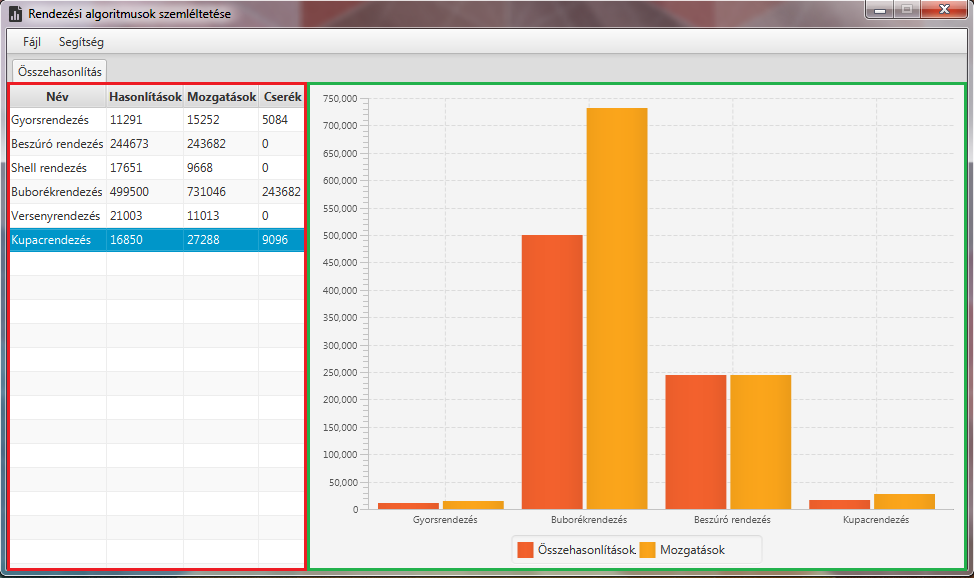
\includegraphics[width=0.8\textwidth]{pics/benchmarkpanel.png}
 	\caption{Összehasonlítás panel}
 \end{figure}
\subsubsection{Elemzés táblázat}
Piros kerettel jelölt rész az ábrán, mely táblázatnak négy oszlopa van:
\begin{description}
	\item[$\bullet$] Név - az algoritmus neve
	\item[$\bullet$] Hasonlítások - a rendezés során végzett összehasonlítások szummája
	\item[$\bullet$] Mozgatások - az elemmozgatások számának összege
	\item[$\bullet$] Cserék - a végzett cserék szummája
\end{description}
A \textbf{Mozgatások} oszlop minden esetben kitöltésre kerül, még ha az algoritmus nem is mozgatásokat használ. Ekkor a mozgatások oszlopban a cserék számának háromszorosa jelenik meg. Ennél fogva egyszerűbb az algoritmusok vizsgálata.
\subsubsection{Elemzés diagram}
A táblázathoz képest balra helyezkedik el a zöld kerettel jelölt oszlopdiagram. Kezdetben teljesen üres, csak a jelölések jelentése látható. Az \textbf{Elemzés táblázat} egy során történő dupla kattintás következtében megjelenik az algoritmus összehasonlításainak és mozgatásainak a száma. Előbbi narancs- utóbbi citromsárga színnel. Amennyiben olyan sorra kattint a felhasználó, mely már látható a diagramon, azon algoritmus adatai eltűnnek a felületről.

\section{A vizsgált algoritmusok}
\subsection{Buborékrendezés}
\subsubsection{Leírás}
A legrégebbi és a legegyszerűbb rendezési algoritmus. Mindemellett a legtöbb esetben a leglassabb is. Már az 1965-ös évben megjelent egy teljes körű elemzése\cite{Demuth}.
\subsubsection{Működés}
 A rendezés minden egyes elemet összehasonlít a rákövetkező elemmel, és ha szükséges megcseréli őket. Ez azt eredményezi, hogy lépésenként a maximális elem "buborék" szerűen a lista végére kerül, ezzel egyidejűleg a kisebb elemek "lesüllyednek" a tömb elejére. Amennyiben egy menetben a maximális eleme elérte a helyét visszavezetjük a problémát az eggyel "rövidebb" rendezési feladatra\cite{Fekete}. Az algoritmus javítható azzal, ha figyeljük, hogy az egyes menetekben történt-e csere. Amennyiben egy olyan menet végére értünk, amelyben egy elem sem cserélt helyet, akkor a tömb már rendezve van. A program az eredeti, nem javított verziót mutatja be.
 \subsubsection{Példa}
 A rendezendő számok: $42, 22, 10, 57$.\par
 Az első ábrán szerepel a kezdeti állapot, a másodikon az első két értéket cseréje látható. A 42 ismét fentebb kerül egy pozícióval a harmadik ábrán. A negyedik ábrán csupán egy összehasonlítás történik, mivel az 57 nagyobb mint az őt megelőző érték. Az ötödik ábrán az előző állapot első két értékének(22 és 10) a cseréje látható. Az ezt követő összehasonlítás eredménye, hogy a második legnagyobb érték(42) a helyére került. Ezt követően már csak egy összehasonlítást történik, mely után az adatsor rendezve lesz.\par
 \begin{figure}[H]
 	\centering
 	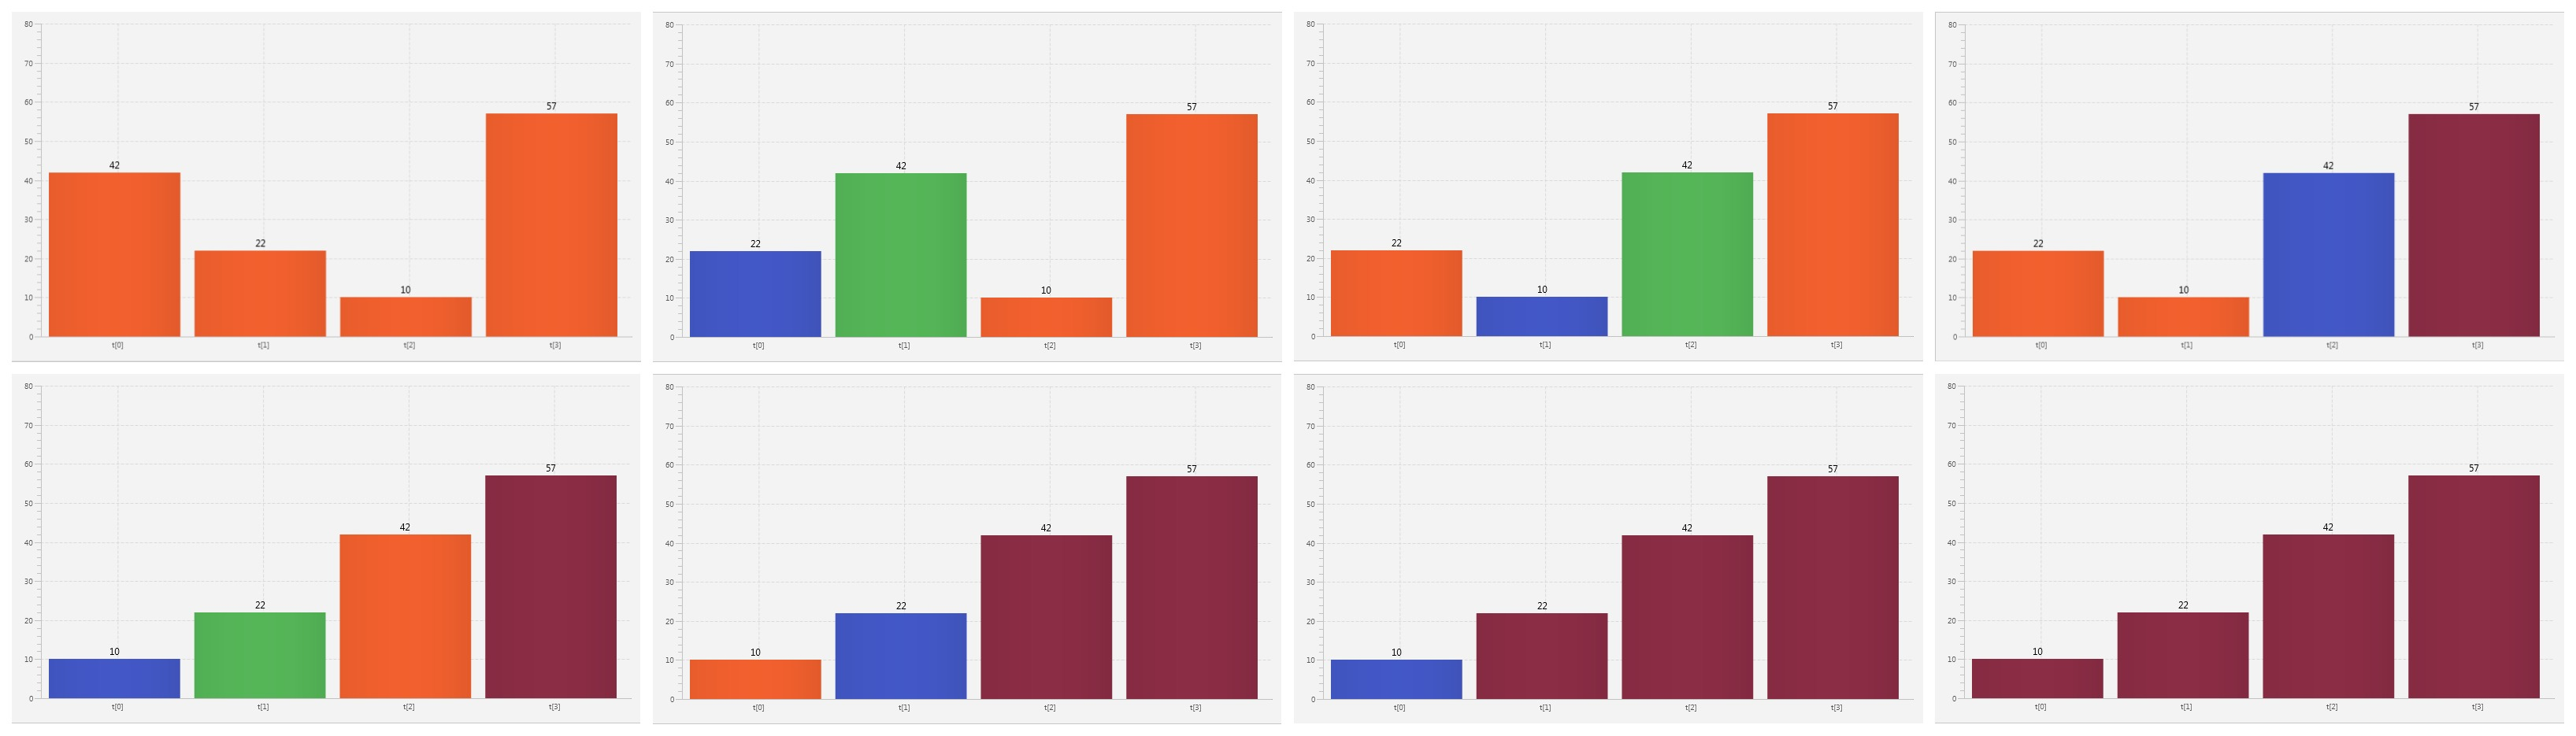
\includegraphics[width=1\textwidth]{pics/bubble.jpg}
 	\caption{Példa a buborékrendezésre}
 \end{figure}\par
 \subsubsection{Műveletigény}
Párosával haladunk végig az elemeken, és így vizsgáljuk őket. Mivel minden menet végén visszavezetjük a problémát az eggyel rövidebb feladatra, ezért az összehasonlítások száma $n$ hosszú bemenetre:\par
$$\ddot{O}(n)=(n-1)+(n-2)+\ldots+1=\frac{n\cdot(n-1)}{2}=\frac{n^2}{2}-\frac{n}{2}=\Theta(n^2)$$
\par A cserék száma már nem állandó, a bemenő adatok inverziószámával egyezik meg. Belátható, hogy minden egyes cserével egy inverzió szüntethető meg két elem között. A legtöbb cserét akkor szükséges eszközölni, ha a rendezendő elemek mindegyike inverzióban áll a rákövetkező elemmel, azaz a tömb nagyság szerint csökkenő sorrendben rendezett. Ekkor a cserék száma:\par
$$MCs(n)=\frac{n\cdot(n-1)}{2}=\Theta(n^2)$$
Amennyiben a tömb elemei már rendezettek, akkor egyetlen cserét sem szükséges végrehajtani.
Az átlagos csereszám a maximális cserék számának fele\cite{Fekete}, ám nagyságrendileg még ez is $\Theta(n^2)$
\subsubsection{Jelölések az állapotjelző felületen}
Kitüntetettnek (\textcolor{select}{\Huge$\bullet$} színnel) jelöljük azt az elemet, amely egy csere következtében feljebb került. Nincs egyéb eltérés az eredeti jelölésekhez képest.

\subsection{Beszúró rendezés}
\subsubsection{Leírás}
 A legtöbb esetben akár kétszer hatékonyabb a buborékrendezéshez képest\cite{Fekete}. Az elve egyszerűen megérthető egy hétköznapi példán keresztül: A kezünkben tartunk kártyalapokat, majd egy pakliból húzva az új lapot beszúrjuk a kezünkben lévő, már rendezett lapok közé. Ennélfogva szokás kártyás rendezésnek is nevezni.
\subsubsection{Működés}
Két részre bontjuk a tömböt, az egyik részén - a tömb bal széle - a már rendezett, míg a másikon a még nem vizsgált elemek szerepelnek. Kezdetben a tömb első elemét tekintjük a rendezett résznek.\par
Lényege, hogy a soron következő elemet - a második elemtől kezdve - egy ideiglenes változóba mentjük, és a rendezett tömbrész elemeit jobbra csúsztatjuk mindaddig, amíg a kiválasztott érték nem kerül a helyére. Ezt n-1 alkalommal ismételve megkapjuk a rendezett tömböt.
 \subsubsection{Példa}
 A rendezendő számok megegyeznek a buborékrendezés bemutatásánál használtakkal, azaz: $42, 22, 10, 57$.\par
 Az első ábrán szerepel a kezdeti állapot. A következő képen jelöljük azt, hogy a második elemet fogjuk beszúrni. A harmadik ábrán felcsúsztatjuk a 42 értéket, majd a negyedik képen már látható, hogy a tömb első két eleme alkotja rendezett tömbrészt. Ezt követően a harmadik elem kerül kiválasztásra. Az összehasonlítások eredményeképp a teljes rendezett tömbrészt jobbra tolódik, így az 7. képen már a tömb első három eleme megfelelő sorrendben van. Végül a tömb utolsó eleme kerül összehasonlításra az őt megelőzővel, mivel nagyobb tőle, így kész a rendezési feladat.\par
 \begin{figure}[H]
 	\centering
 	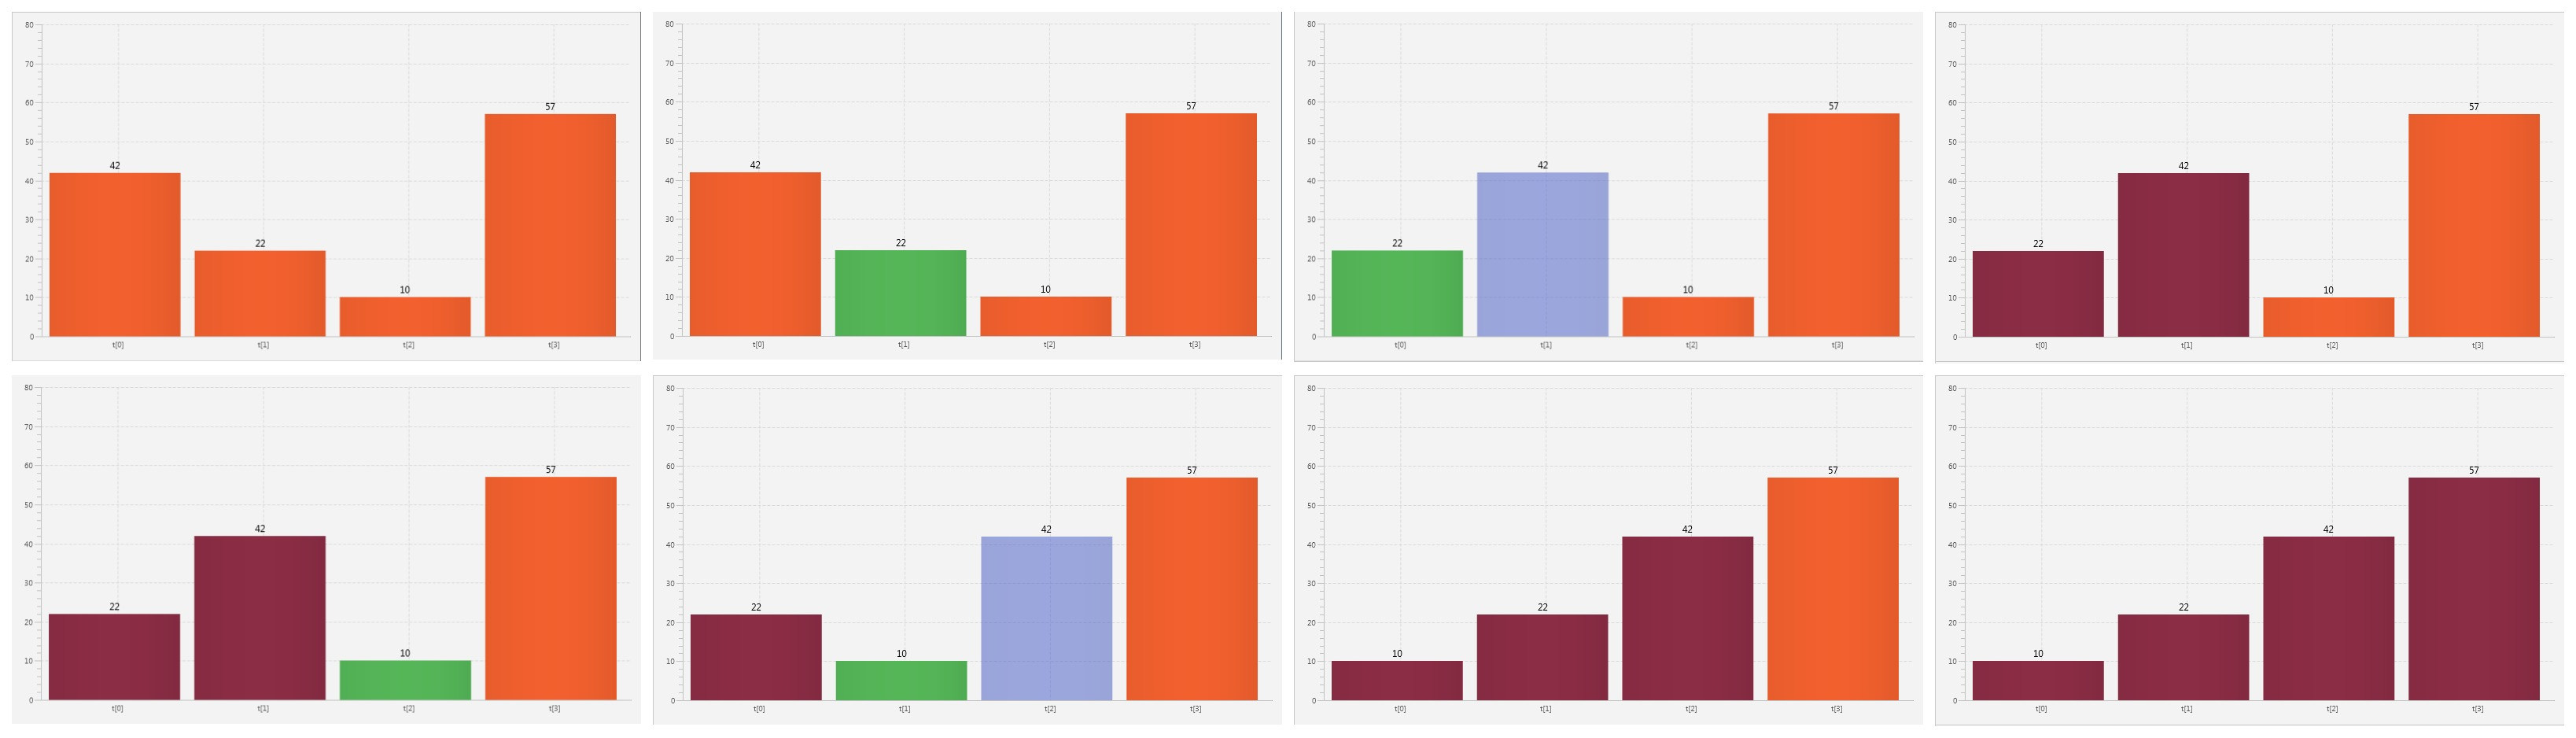
\includegraphics[width=1\textwidth]{pics/insertion.jpg}
 	\caption{Példa a beszúró rendezésre}
 \end{figure}\par
\subsubsection{Műveletigény}
Legjobb esetben elegendő a második elemtől mindegyik elemet az előtte található értékkel összehasonlítani, vagyis a tömb már eleve rendezett. Ez pontosan n-1 összehasonlítást jelent, azaz:
$$m\ddot{O}(n)=(n-1)=\Theta(n)$$
Ebben az esetben pedig egyetlen elemet sem kell mozgatni.\par
A legrosszabb eset akkor áll fenn, ha a beszúrandó elem minden alkalommal kisebb a már beszúrt elemeknél, azaz a tömb elemei csökkenőleg rendezettek. Ekkor az összehasonlítások száma:
$$M\ddot{O}(n)=\sum\limits_{i=1}^n i = \frac{(1+(n-1))\cdot(n-1)}{2}=\frac{n\cdot(n-1)}{2}=\Theta(n^2)$$
Továbbá ekkor a mozgatások száma:
$$MM(n)=\Theta(n^2)$$
\subsubsection{Jelölések az állapotjelző felületen}
A már rendezett tömbrészt \textcolor{done}{\Huge$\bullet$} szín jelöli. Az aktuálisan beszúrandó elem pedig a \textcolor{select}{\Huge$\bullet$} jelölést kapja. A kiválasztott elemmel összehasonlított értékek \textcolor{swap}{\Huge$\bullet$} színt kapnak.\par
Megjegyzendő, hogy a kitüntetett szerepű avagy beszúrandó elem nem szerepel tömbelemként az összehasonlításkor, csupán a felületen van jelölve a jobb megérthetőség okán.

\subsection{Shell rendezés}
\subsubsection{Leírás}
\textbf{Donald Shell} nevéhez fűződik, a legtöbb esetben a leggyorsabb négyzetes idejű algoritmus. Az elve az, hogy célszerű lehet előbb a "távolabb" lévő elemeket hasonlítani és mozgatni, mivel így az elemek hamarabb közel kerülhetnek a végleges helyükhöz.
\subsubsection{Működés}
Többször vizsgálja a tömböt, és minden alkalommal egy részén beszúró rendezést hajt végre. Arra, hogy mekkora méretű résztömböt vizsgáljon az egyes lépésekben az algoritmus több javaslat is található. A teljesség igénye nélkül néhány ajánlás\cite{ShellWiki} erre vonatkozóan:\par
\begin{table}[h]
	\def\arraystretch{2}
	\centering
	\begin{tabular}{|c|c|c|c|}
		\hline
		\textbf{Szabály (k=1...)} & \textbf{Konkrét értékek}  & \textbf{Műveletigény} & \textbf{Szerző}         \\ \hline
		$\lfloor n / 2^k \rfloor$&      $\left\lfloor\frac{n}{2}\right\rfloor,
		\left\lfloor\frac{n}{4}\right\rfloor, \ldots$, 1            &              $\Theta(n^2)$                      & Shell, 1959     \\ \hline
		$2^k-1$&      1, 3, 7, 11, $\ldots$           &              $\Theta(n^\frac{3}{2})$                      & Hibbard, 1963    \\ \hline
		$2^p 3^q$ váltakozva & 1, 2, 3, 4, $\ldots$  &               $\Theta(n \log^2 n)$                     & Pratt, 1971     \\ \hline
	\end{tabular}
\end{table}
 \subsubsection{Példa}
 Az előző példákban használt számokat kívánjuk rendezni ismét, azaz a bemenet: $42, 22, 10, 57$.\par
 Az első képen látható a kezdeti állapot. A következő ábrán jelöljük azt, hogy a harmadik elemet fogjuk mozgatni, ekkor a lépésköz kettő. A harmadik képen látható az első elem átmozgatása, a kiválasztott elemet beszúrjuk a helyére. A negyedik képen vesszük a következő elemet, továbbra is 2 lépésközzel megvizsgáljuk a második indexen lévő elemet az ötödik ábrán. Itt nem történik mozgatás. Végül a hatodik megjelenített lépéstől kezdve beszúró rendezést alkalmazunk.\par
 \begin{figure}[H]
 	\centering
 	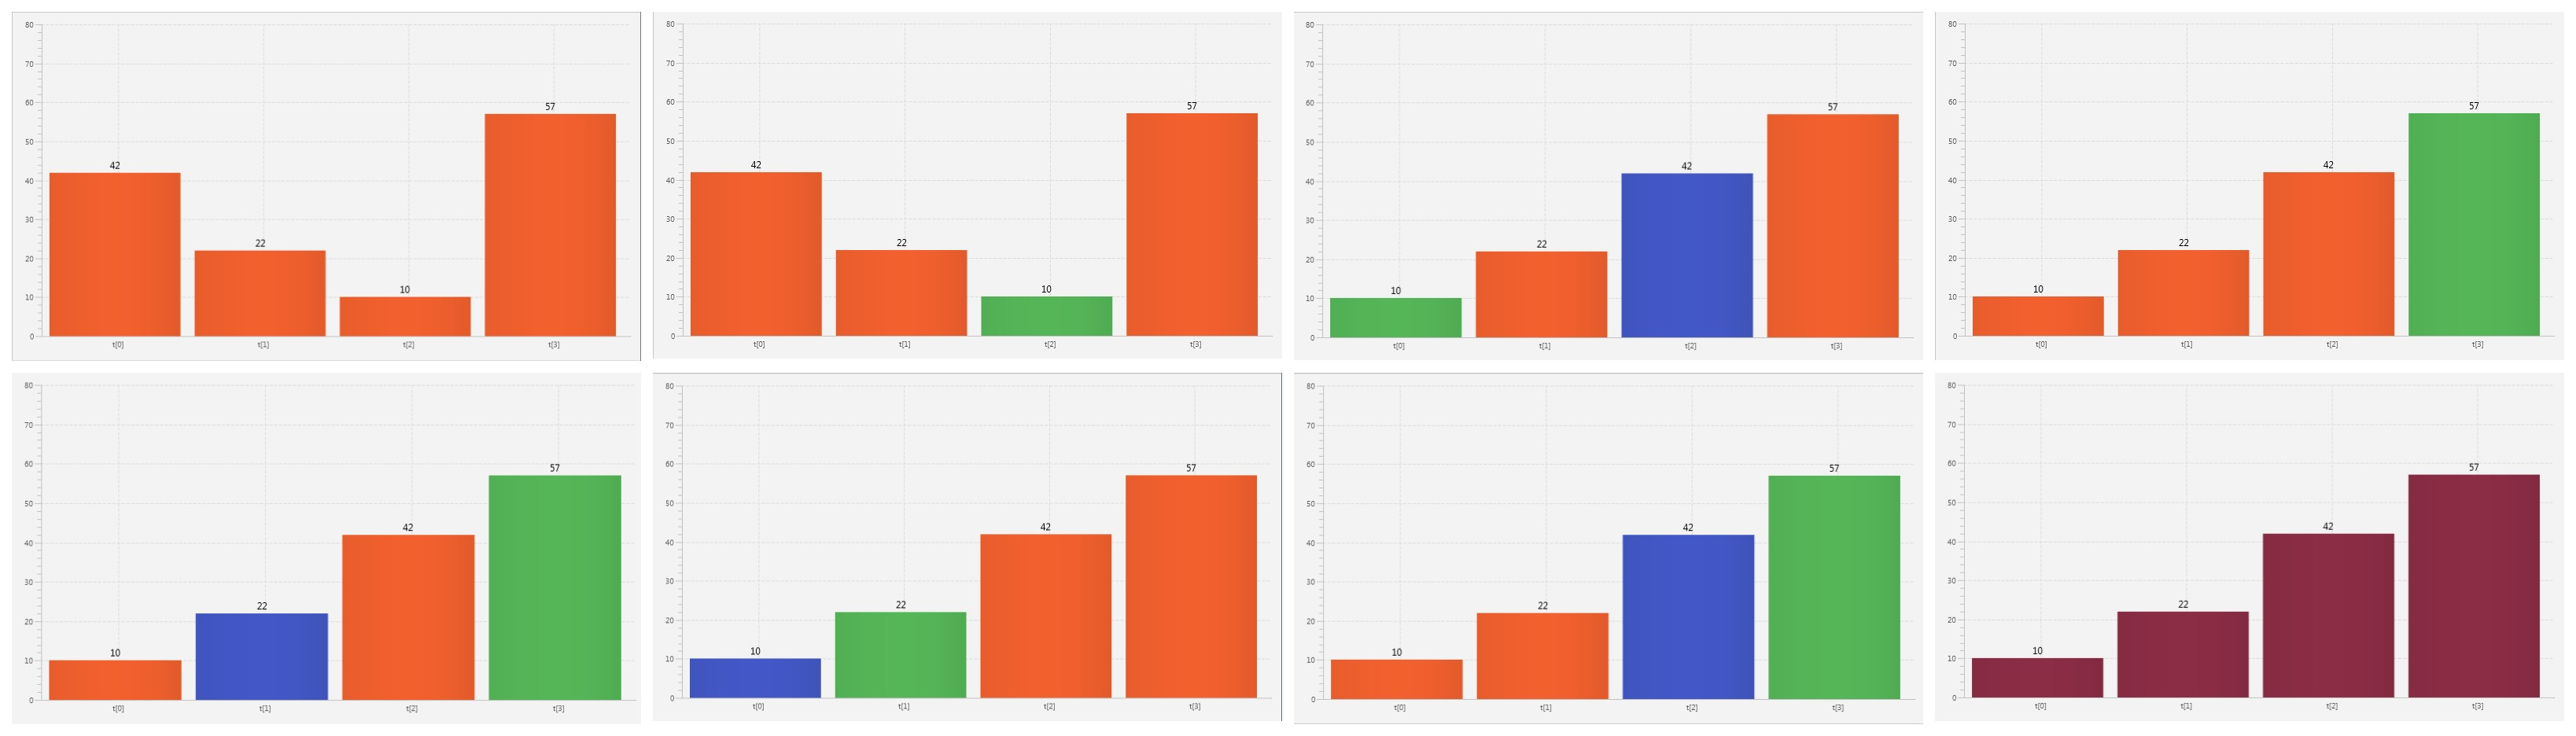
\includegraphics[width=1\textwidth]{pics/shell.jpg}
 	\caption{Példa a Shell rendezésre}
 \end{figure}\par
\subsubsection{Műveletigény}
 A fentebbi táblázatból látható, hogy az algoritmus sebessége nagyban függ a lépésköz megválasztásától. A program a legrégebbi, \textbf{Donald Shell} által javasolt értékeket\cite{Shell} használja, így legrosszabb esetben $\Theta(n^2)$ a műveletek száma.\par
 A legjobb eset akkor áll fenn, ha a tömb elemei már rendezettek, ekkor nincs szükség mozgatásra, az algoritmus futási ideje $\Theta(n)$ nagyságrendű.
\subsubsection{Jelölések az állapotjelző felületen}
 A felület bemutatásában szereplőkhöz képest nincs eltérés.

\subsection{Gyorsrendezés}
\subsubsection{Leírás}
\textbf{C.A.R. Hoare}\cite{Horae} alkotta meg 1965-ben. Az egyik leggyorsabb rendezési eljárás, ezért rendkívül gyakran alkalmazzák.
\subsubsection{Működés}
Helyben rendező, oszd meg és uralkodj\cite{Cormen} elven működő rekurzív algoritmus. A következő négy lépésre bontható fel az rendezés:
\begin{description}
	\item[$\bullet$] Ha csak egy vagy nulla elemű az elemzett rész, akkor ne tegyünk semmit.
	\item[$\bullet$] Válasszunk egy vezérelemet (legjobb oldalibb elem).
	\item[$\bullet$] Osszuk két részre a rendezendő részt, az egyik oldalára a vezérelemtől kisebb, míg a másikra a nagyobb elemek kerüljenek.
	\item[$\bullet$] Rekurzívan ismételjük meg az előbbi lépéseket a résztömbökön.
\end{description}
Gyakorlatilag szétválasztást eszközölünk, melynek eredményeképp a kiválasztott elemtől kisebb értékek tőle balra, a nagyobbak pedig jobbra helyezkednek el. Az egyszerűbb megérthetőséget szem előtt tartva a program mindig a legjobboldalibb elemet szelektálja.
 \subsubsection{Példa}
 Az eddigi példákkal megegyezően a bemenet: $42, 22, 10, 57$.\par
 Az első képen látható a már kiválasztott vezérelem. A negyedik ábráig csak összehasonlítások történnek, mivel minden elem kisebb, mint a kiválasztott érték. A negyedik képen a három elemű résztömbön végezzük el a rendezést, a vezérelem ismét a legjobboldalibb érték. Az ötödik képen az első érték nagyobb mint a vezérelem, így ezt az elemet a hatodik képen megcseréljük a vezérelemmel. Ezt követően a középső két elem kerül összehasonlításra, mivel nincs szükség cserére így a rendezés befejeződött.\par
 \begin{figure}[H]
 	\centering
 	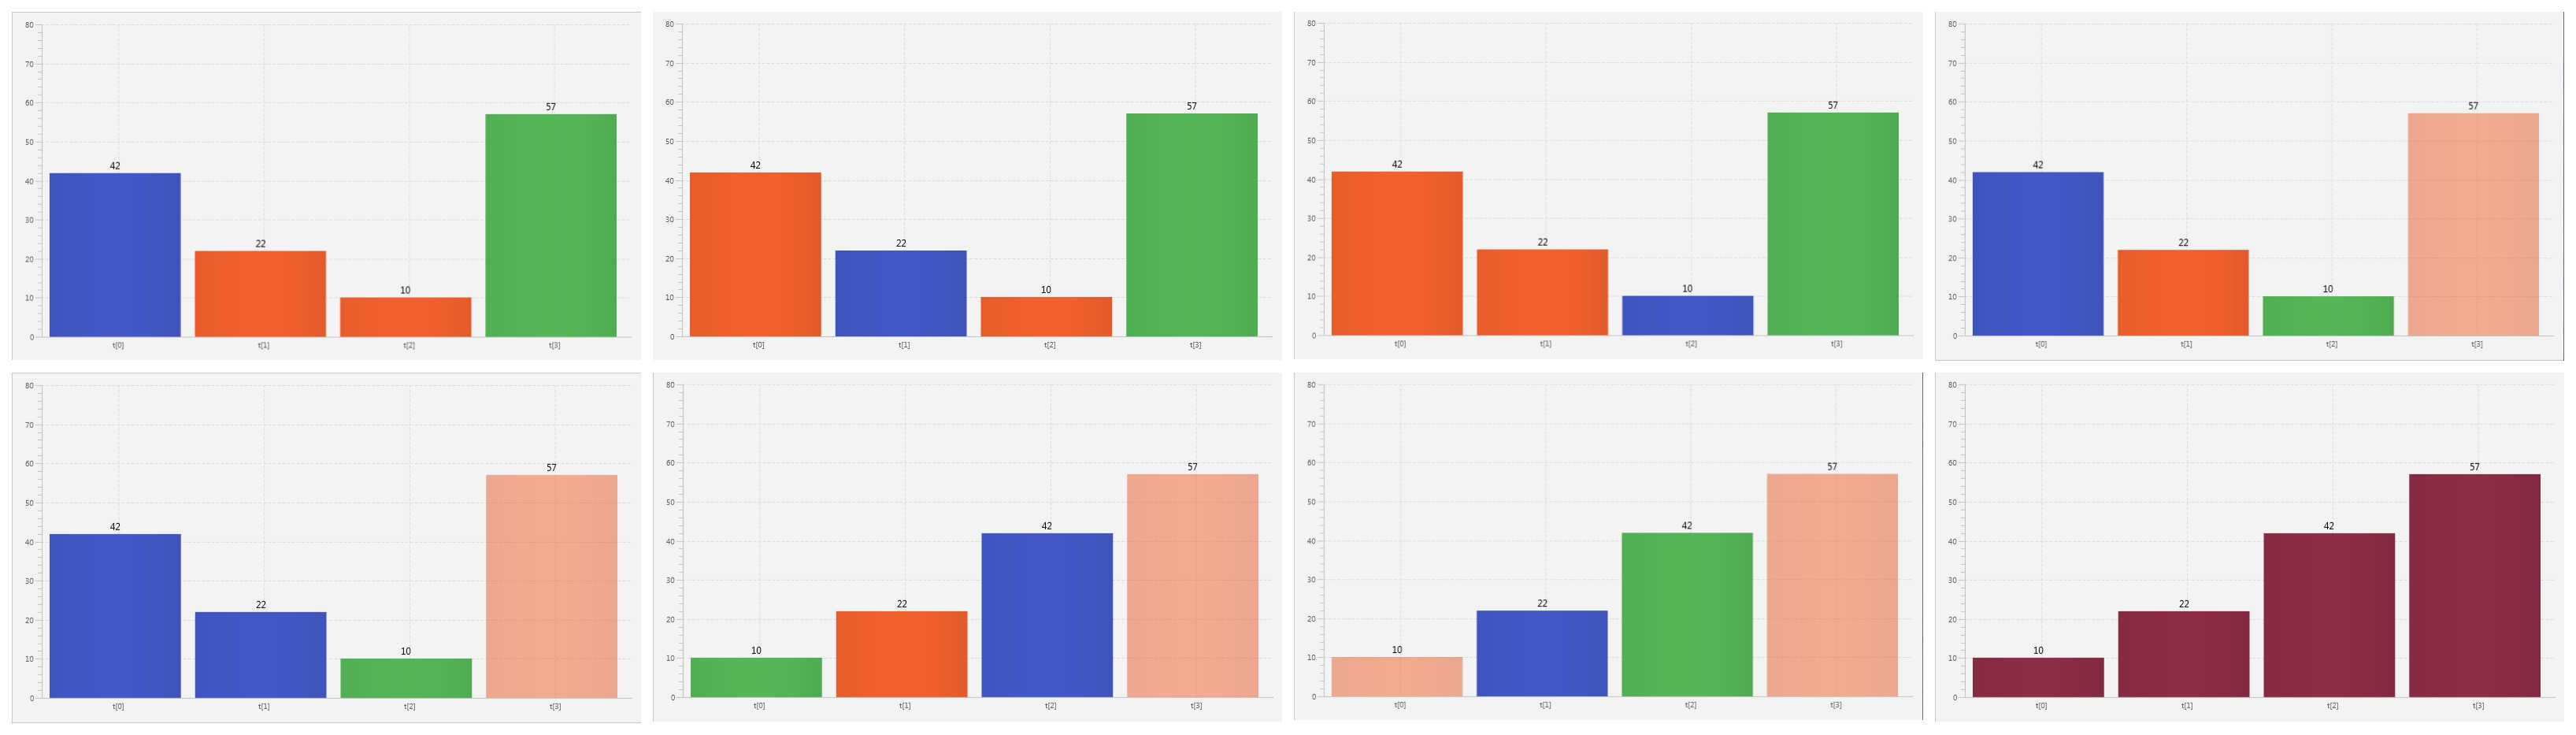
\includegraphics[width=1\textwidth]{pics/quick.jpg}
 	\caption{Példa a gyorsrendezésre}
 \end{figure}\par
\subsubsection{Műveletigény}
A rendezés műveletigényét befolyásolja, hogy hogyan választjuk meg a vezérelemet. Például a legrosszabb futási időt ($\Theta(n^2)$) eredményezi, ha mindig a legjobboldalibb elemet választjuk vezérelemnek, és a tömb elemei csökkenő sorrendben vannak\cite{Cormen}. Éppen ezért a gyakorlatban javasolt ezen elem véletlenszerű megválasztása.\par
Ha feltételezzük azt, hogy minden rekurzív lépés felezi a tömböt, akkor egy $n\log(n)$ magasságú fával lehet ábrázolni a rekurziót. Továbbá, mivel minden szinten az elemek száma $n$, és ezek particionálásához használt lépésszám $\Theta(n)$ így a legjobb esetben a futási idő $\Theta(n\cdot\log(n))$.\par
 A gyorsrendezés a legtöbb esetben(közepes és nagy méretű bemenetre) a legmegfelelőbb választás ha számít a rendezés sebessége, mivel az átlagos futási ideje - $\mathcal{O}(n\cdot\log(n))$ - közel áll a legjobb futási időhöz\cite{Cormen}.\par
 Amennyiben a tömb elemei már eleve rendezettek vagy esetleg fordított sorrendben szerepelnek nem hatékony az eljárás.
\subsubsection{Jelölések az állapotjelző felületen}
A vezérelemet \textcolor{select}{\Huge$\bullet$} szín jelöli. Annak érdekében, hogy jobban átlátható legyen, hogy éppen melyik résztömbön folyik a vizsgálat az éppen nem vizsgált rész haloványabb sárga színnel van jelölve. A többi jelölés a felület bemutatásában leírtaknak megfelelően történik.

\subsection{Kupacrendezés}
\subsubsection{Leírás}
Az $\mathcal{O}(n\log (n))$ algoritmusok közül az egyik leglassabb, azonban előnye a gyorsrendezéssel szemben, hogy nem erőteljesen rekurzív. Ennél fogva jól alkalmazható milliós nagyságrendű bemenetre. Ahogyan a neve is sugallja, a rendezéshez egy kupac adatszerkezetet használ. Az algoritmus ismertetése előtt definiáljuk a kupac fogalmát\cite{Fekete}:
Olyan bináris fa, amelyre a következők teljesülnek:
\begin{description}
	\item[$\bullet$] Kizárólag a levelek szintjén hiányozhat csúcs, azaz "majdnem teljes".
	\item[$\bullet$] A levélszint csúcsai balra tömörítettek.
	\item[$\bullet$] Minden belső csúcs értéke nagyobb vagy egyenlő, mint a gyerekeinek értékei.
\end{description}
A második pont értelmében egyetlen olyan csúcs lehet, amelynek csak egy gyereke van, és az közvetlenül a levélszint felett kell, hogy elhelyezkedjen.\par
\subsubsection{Működés}
A rendezés az előbbi tulajdonságokra támaszkodik. 
Az algoritmus a bemeneti elemekből kupacot épít, majd a legfelsőbb elemét áthelyezi a kupac "végére". Ezt követően ellenőrzi a kupac tulajdonságokat, ahol szükséges cseréket hajt végre, hogy helyreálljon a kupac adatszerkezet, ekkor már az utolsó, legjobboldalibb levélelem nem vesz részt a kupacépítésben. A gyökérben található elemet a legjobboldalibb levélelem elé helyezi, és újraépíti a kupacot. Ezen lépések addig ismétlődnek, amíg már a maximális elem áthelyezése nem lehetséges, a kupac "végére" helyezési művelet elérte a gyökeret.\par
 \subsubsection{Példa}
 Az eddigi példákkal azonosan a rendezendő számsorozat: $42, 22, 10, 57$.\par
 Az első kép a kezdeti állapotot mutatja. Ezt követően a bemeneti adatokból kupacot építünk, melynek eredménye a második ábra. A gyökérelemet a levélszint utolsó elemével megcseréljük a harmadik képen. Ellenőrizzük, hogy teljesülnek-e a kupac tulajdonságok, amennyiben nem cseréket hajtunk végre, ennek eredménye látható a 4. képen. Ismét a gyökérelemet lesüllyesztjük, majd ellenőrizzük a kupac tulajdonságot. Az előző két lépést megismételve rendezett tömböt kapunk.\par
 \begin{figure}[H]
 	\centering
 	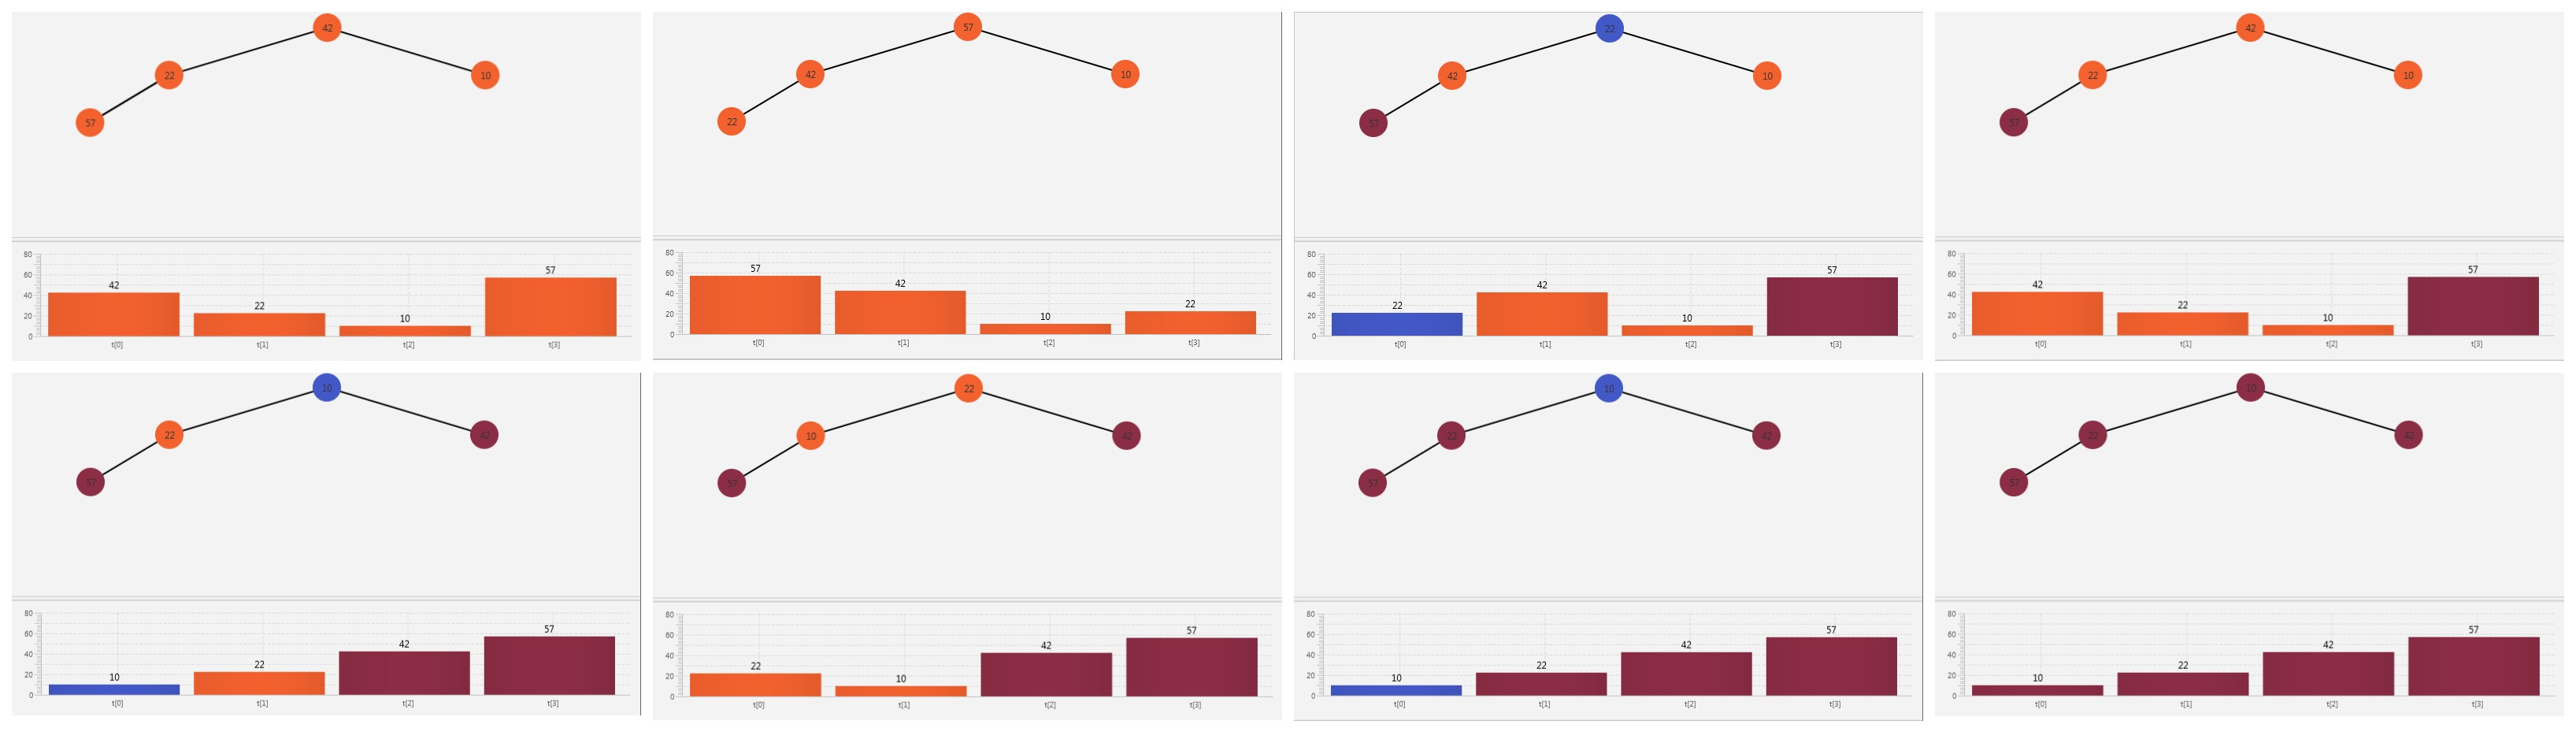
\includegraphics[width=1\textwidth]{pics/heap.jpg}
 	\caption{Példa a kupacrendezésre}
 \end{figure}\par
\subsubsection{Műveletigény}
A kupacrendezés egyik további, hogy míg a gyorsrendezésnek legrosszabb esetben a futási ideje $\mathcal{O}(n^2)$, addig itt a futási idő továbbra is $\mathcal{O}(n\cdot\log (n))$. Ennél fogva azon rendszereknél, ahol a négyzetes futási idő elfogadhatatlan inkább kupacrendezést alkalmaznak.
\subsubsection{Jelölések az állapotjelző felületen}
Az éppen összehasonlított értékeket \textcolor{swap}{\Huge$\bullet$} jelöli. Amennyiben csere történt a belső csúcsba kerülő érték háttérszíne \textcolor{select}{\Huge$\bullet$} lesz. Ez alól kivétel, ha a gyökérbe került új érték, mivel ekkor már tudjuk az új legnagyobb értéket, ennek a színe \textcolor{done}{\Huge$\bullet$} lesz. Továbbá akkor is ezt a színt használjuk, ha már a tényleges, végleges helyére került egy elem.

\subsection{Versenyrendezés}
\subsubsection{Leírás}
A maximum-kiválasztó rendezések közé tartozik, minden egyes menetben kiválasztja a legnagyobb elemet, kiírja és végül eltávolítja. A maximum kiválasztásnak a gyakorlati hátterét a sportesemények lebonyolítási rendje adja, azaz meghatározza az elemek között a "nyertest"\cite{Fekete}. A módszert n=2$^k$ inputhossz esetén érdemes alkalmazni, mivel ettől értérő bemenetre sokkal kedvezőbb eredményt lehet elérni a kupacrendezéssel\cite{Fekete}. \par
\subsubsection{Működés}
Az algoritmus által használt adatszerkezet egy teljes bináris fa. A bináris fa leveleiben szerepelnek a rendezendő elemek. Az első speciális menetben a fa belső pontjait kitöltjük, úgy, hogy a pontba a gyerekei közüli nagyobb érték kerül.\par 
Ezt követően kerül sor az $(n-1)$ egyszerűbb menetre: A gyökérben található elemet keresve "lefelé" haladunk a bináris fában, majd megtalálva azt a levelet amelyben a gyökér értéke szerepel egy abszolút vesztest állítunk a helyére. Ez az érték a programban -1, mivel csak pozitív egészeket használunk a rendezések szemléltetésére. Ezzel ellentétben a gyakorlatban ez az érték $-\infty$. Majd ezen az "ágon" újrajátsszuk a mérkőzéseket.\par
Amennyiben a bemenet hossza nem kettő hatvány a program -1 értékekkel tölti fel a bináris fa további leveleit, amíg a bemenet hossza nem lesz megfelelő.
 \subsubsection{Példa}
 Az eddigi példákkal megegyezően a bemenet: $42, 22, 10, 57$.\par
 Az első ábra a kezdőállapotot mutatja. A második kép a versenyfa kitöltését követő állapot, melynek eredményeképp megjelenik az abszolút maximum érték a diagramon. Ezt követően a harmadik képen látható a maximális értékhez tartozó levélelem megtalálásának állapota. A negyedik ábra szemlélteti az újrajátszás eredményét. Az előzőekhez hasonlóan szemléltetik a további képek a maximum érték megjelenítését, a levélelem megkeresését majd az újrajátszás eredményét.\par
 \begin{figure}[H]
 	\centering
 	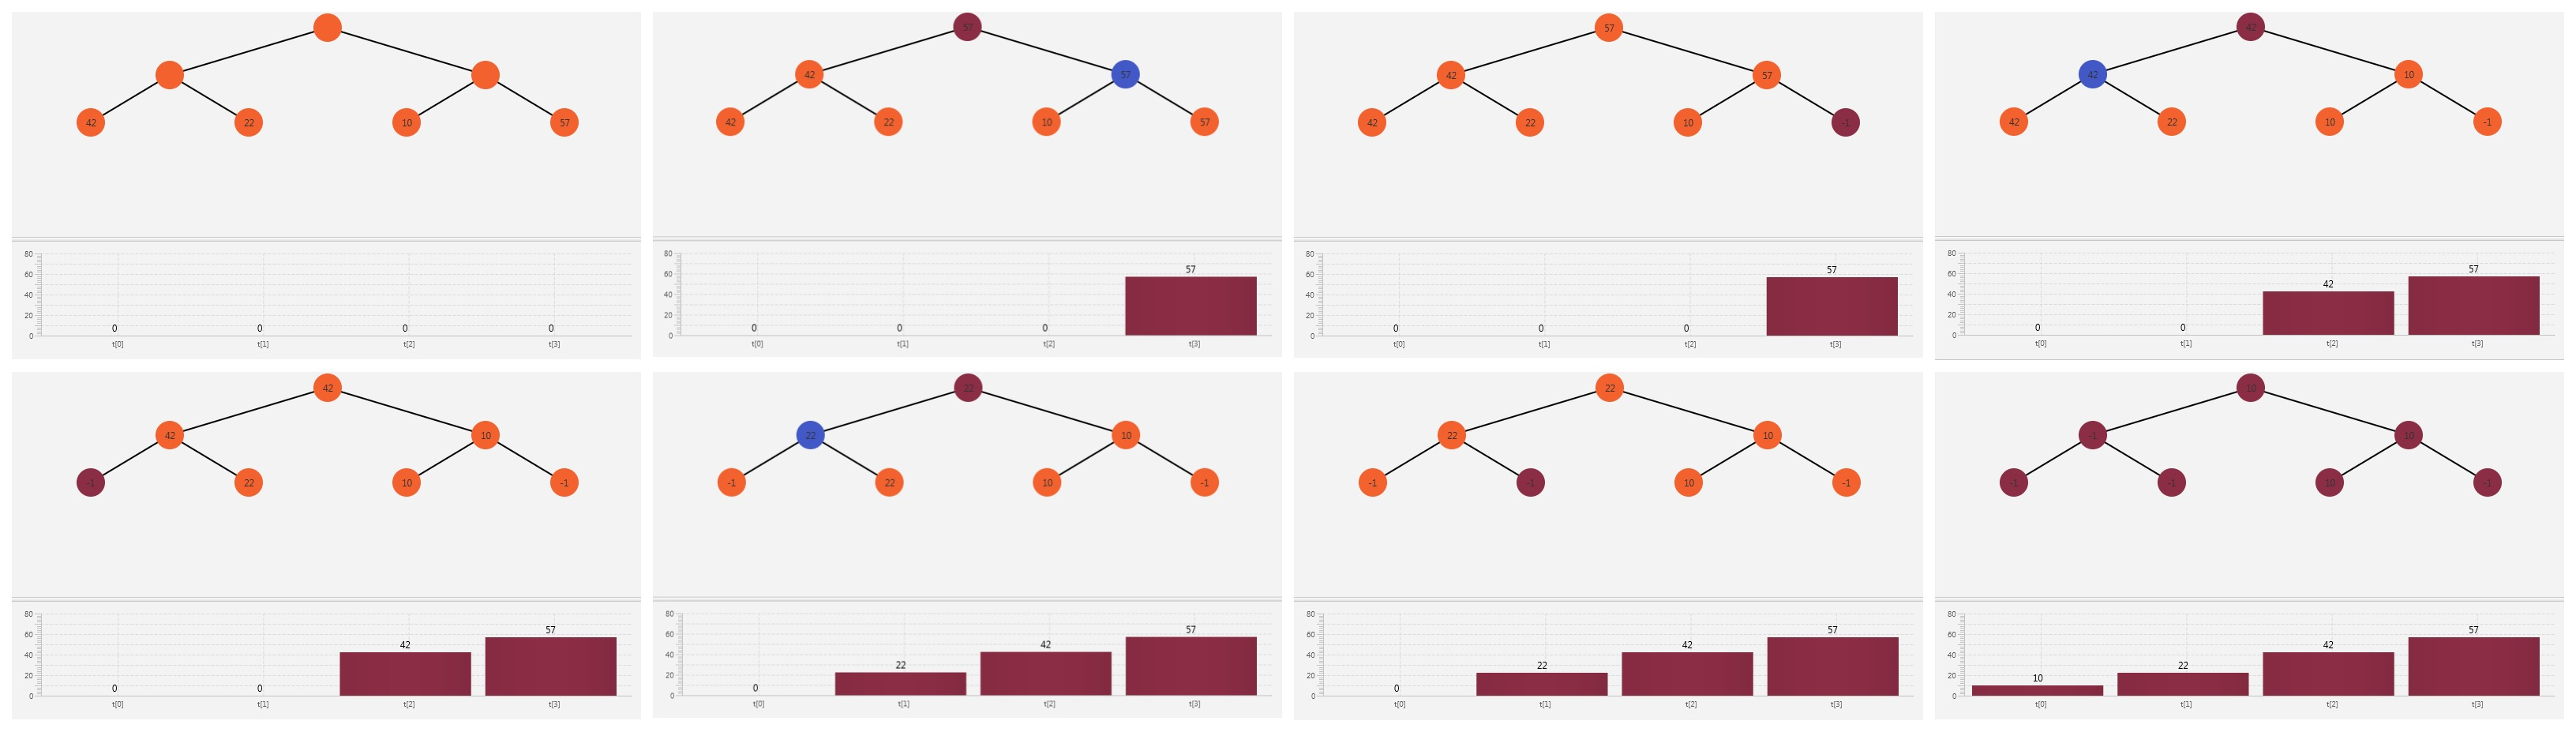
\includegraphics[width=1\textwidth]{pics/tournament.jpg}
 	\caption{Példa a versenyrendezésre}
 \end{figure}\par
\subsubsection{Műveletigény}
A rendezés egyetlen hátránya a tárigénye, $n$ szám esetén további $n-1$ mezőre szükség van a versenyfa elkészítéséhez. Éppen emiatt a gyakorlatban nem sűrűn használt eljárás. Az első, speciális menet, a versenyfa kitöltése $n-1$ összehasonlítást és mozgatást használ ($n-1$ a belső csúcsok száma). Minden további menetben a fán kétszer kell végigmenni, melynek magassága $\log_2(n)$. Egyszer a maximális levél megtalálásához, majd az újrajátszáshoz, így a ezen menetek $2\log_2(n)$ összehasonlítást végeznek. Mozgatás csak a második, újrajátszási művelethez tartozik. Így a műveletigények:
$$\ddot{O}(n)=n-1+(n-1)\cdot2\cdot\log_2(n)=\Theta(n\cdot(\log(n))$$
$$M(n)=n-1+(n-1)\cdot\log_2(n)=\Theta(n\cdot(\log(n))$$
\subsubsection{Jelölések az állapotjelző felületen}
Az összehasonlításokat, valamint a maximális levélelem megkereséséhez bejárt utat \textcolor{swap}{\Huge$\bullet$} szín jelöli. A meccsek lejátszásakor a belső csúcsba kerülő érték \textcolor{select}{\Huge$\bullet$} jelölést kap. Ez alól kivétel, amikor a gyökérbe kerül egy meccs győztese, ekkor \textcolor{done}{\Huge$\bullet$} lesz az elem színe, továbbá akkor is ez a jelölés, amikor megtaláltuk a maximális levélcsúcsot.

\subsection{Radix "előre"}
\subsubsection{Leírás}
Az előzőekben ismertetett algoritmusok mindegyike összehasonlításon alapuló rendezés. A radix rendezés viszont az edényrendezések közé tartozik. Ezen rendezések nem hasonlítják össze az elemeket, hanem az elemek az értéküknek megfelelő edényekbe kerülnek. Az edényrendezések eredményeként rendezett adatsorozatot kapunk lineáris időben. 
A radix rendezés egy rekurzív algoritmus, melynek minden szintjén létrejönnek az edények.\par
Az általános edényrendezés egy speciális változata a radix előre rendezés, bináris, $d$ hosszú számokra.\par
\subsubsection{Működés}
Az első menetben a rendezendő elemek első bitjét vizsgálja az algoritmus. A vizsgálat két mutatóval történik, melyek a tömb két végéről indulnak. A tömb elején addig halad a mutató, amíg a vizsgált elem első jegye nem 1, ezzel párhuzamosan a tömb végén olyan elemet keres a másik, melynek első jegye 0. Amennyiben talált ilyen elemeket megcseréli őket. Ezt mindaddig folytatódik, amíg a két mutató nem találkozik. Ekkor kialakul két edény, az elsőben a 0-ás kezdőbittel rendelkező számok, míg a másodikban az 1-essel kezdődő elemek foglalnak helyet. Ezt követően a második bit kerül vizsgálatra az "aledényekben", az előzővel azonos módon. A rendezés befejeződött, ha minden számjegy szerinti vizsgálat megtörtént, vagy ha mindegyik, a futás alatt kialakult edény már csak egy elemet tartalmaz.
 \subsubsection{Példa}
 Az rendezendő számok: $2, 3, 1, 3$, azaz binárisan $10, 11, 01, 11$.\par
 Az első ábra a kezdőállapotot mutatja. Mivel az első érték valószínűleg nem megfelelő helyen van, ezért a tömb végéről kezdve keresünk egy olyan értéket, amely 0-ás jeggyel kezdődik. A harmadik elem pont ilyen, a második képen ez a két érték cserére van kijelölve, majd a negyedik ábrán megtörténik a két elem cseréje. Az ötödik képen látható a menet során kialakult két edény. Mivel az első edény egy elemű, így nem szükséges a vizsgálata. A második edényben az 10 értéket szeretnénk cserélni, így az edény végétől haladunk előrefelé, amíg nem találunk olyan elemet, melynek második bitje egy. A 11 érték éppen ilyen, ezért megcseréljük őket. Az utolsó ábrán látható a rendezett sorozat.\par
 \begin{figure}[H]
 	\centering
 	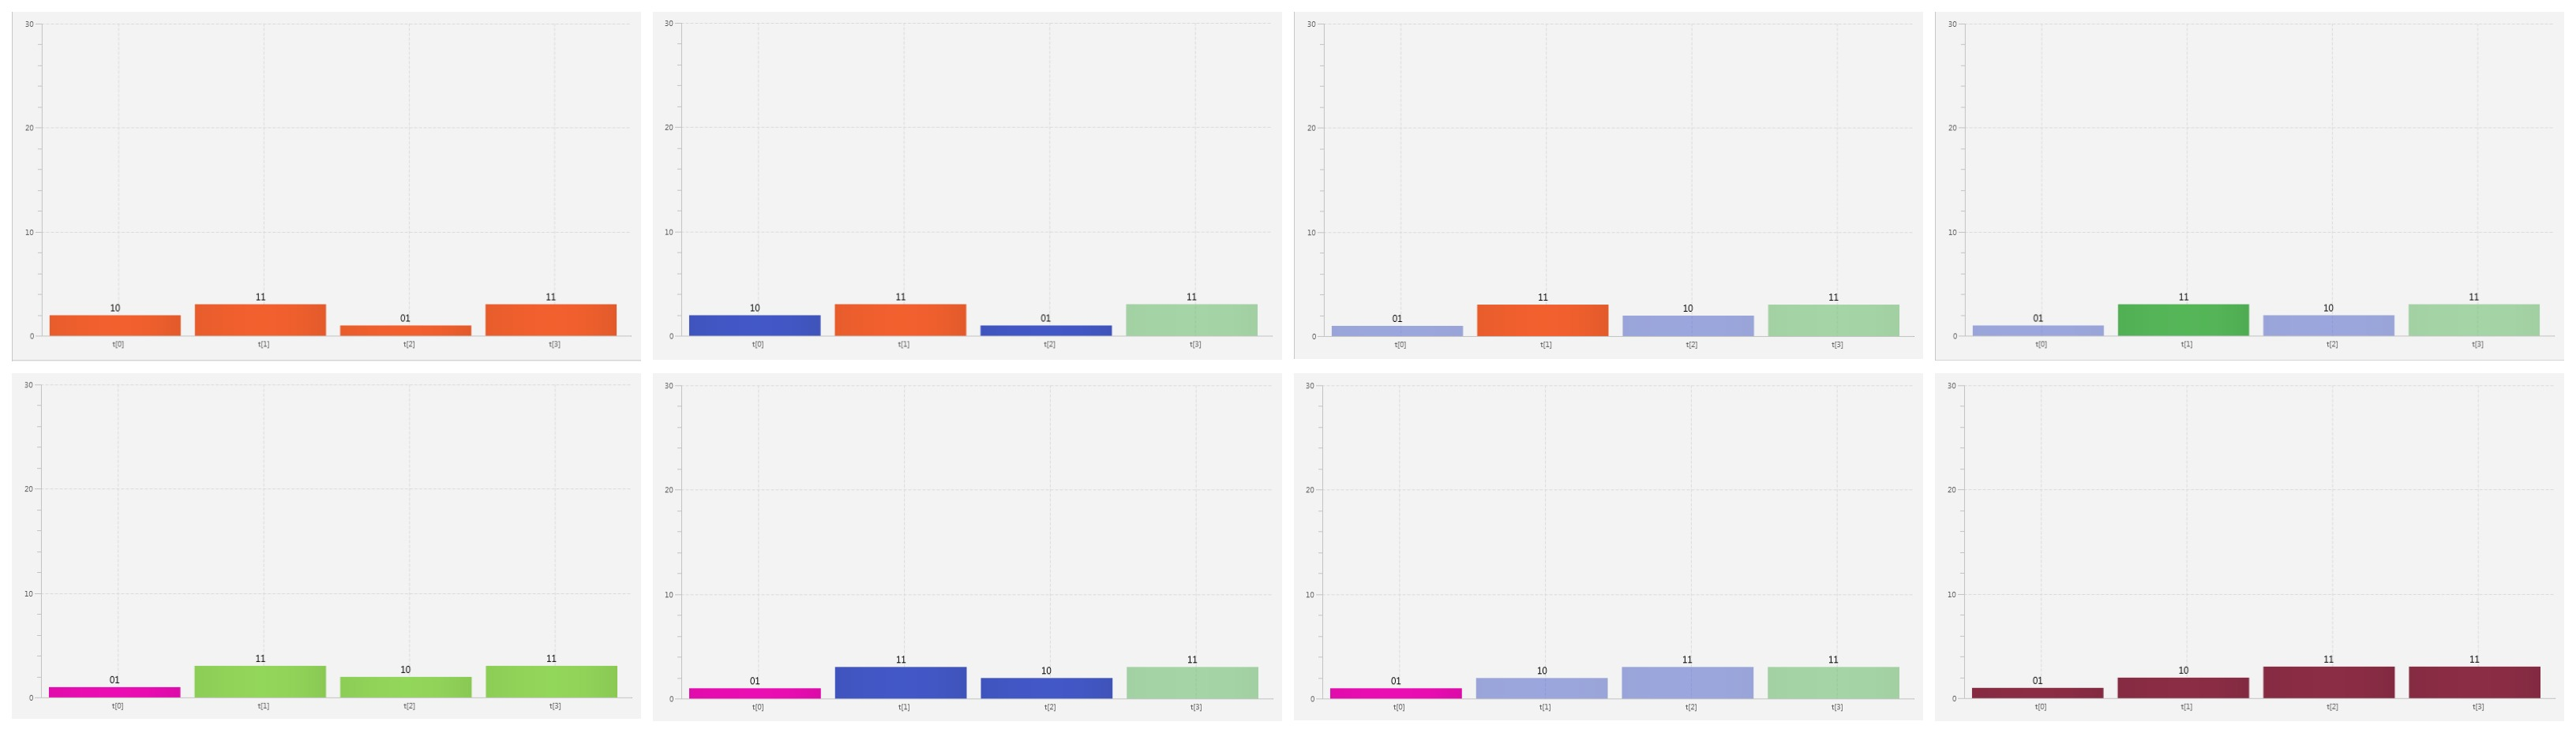
\includegraphics[width=1\textwidth]{pics/radixforward.jpg}
 	\caption{Példa a radix "előre" rendezésre}
 \end{figure}\par
\subsubsection{Műveletigény}
A rendezés lineáris időben történik, a számjegyek számát jelölje $d$, ekkor belátható, hogy a legrosszabb esetben is, azaz ha az összes szám minden bitjét meg kell vizsgálnunk az algoritmus futási ideje:
$$T(n)=\Theta(d \cdot n) = \Theta(n)$$
\subsubsection{Jelölések az állapotjelző felületen}
Az éppen vizsgált elem \textcolor{select}{\Huge$\bullet$} színnel van jelölve. Amennyiben két elemet fel kell cserélni \textcolor{swap}{\Huge$\bullet$} háttérszínt kapnak. Továbbá a már vizsgált elemek háttérszíne fakóbb lesz. Amennyiben egy új edény keletkezik annak a színe véletlenszerűen választódik ki.

\subsection{Radix "vissza"}
\subsubsection{Leírás}
Az algoritmus rövid ismertetője megegyezik a \textbf{Radix "előre"} rendezés leírásával.
\subsubsection{Működés}
Az előző algoritmustól eltérően már nem helyben rendez, az eljárásnak két tömbre van szüksége. További különbség, hogy a kisebb helyiértéktől a nagyobb felé halad a vizsgálat.\par Amennyiben az aktuálisan vizsgált bit értéke 0, akkor a "második" tömb elejére, ellenkező esetben a tömb végére töltjük át az aktuális bináris számot. Ezáltal minden egyes menetben két edény keletkezik: egy, melyben található számok aktuális bitje 0, s egy másik, melyek vizsgált számjegye 1-es. Ezt követően a 0-ás edényt az elejéről olvasva feltöltjük újra az eredeti tömböt az előbb ismertetett módon, majd a 1-es edényt elemeit az utolsó elemtől visszafelé haladva töltjük át az értékeket.
 \subsubsection{Példa}
 A bemenet megegyezik a radix "előre" példájában használt számokkal, azaz: $2, 3, 1, 3$, amelyek binárisan a $10, 11, 01, 11$ értékek.\par
 Az első ábra a kezdeti állapotot mutatja. A második képen a tömb első két eleme már áttöltésre került, a 10 az alsó tömb elejére, míg a 11 a végére. A harmadik ábrán látható a teljen áttöltött állapot. A következő ábrán visszatöltésre került az első érték, melynek első bitje 1, így az eredeti tömb végére került. Ekkor a második edény értékeit hátulról előrefelé vizsgáljuk, így a 10 érték kerül először az eredeti tömb elejére, majd a 11 a 10 előtti helyre. Végül az utolsó 11-es érték is bekerül az eredeti tömbbe. Ezt követően az 5. ábrán már csak átmásolásra kerülnek az értékek a megfelelő sorrendben, azaz az egyes edény tartalma előröl olvasva, míg a második edény értékei hátulról előrefelé haladva. \par
 \begin{figure}[H]
 	\centering
 	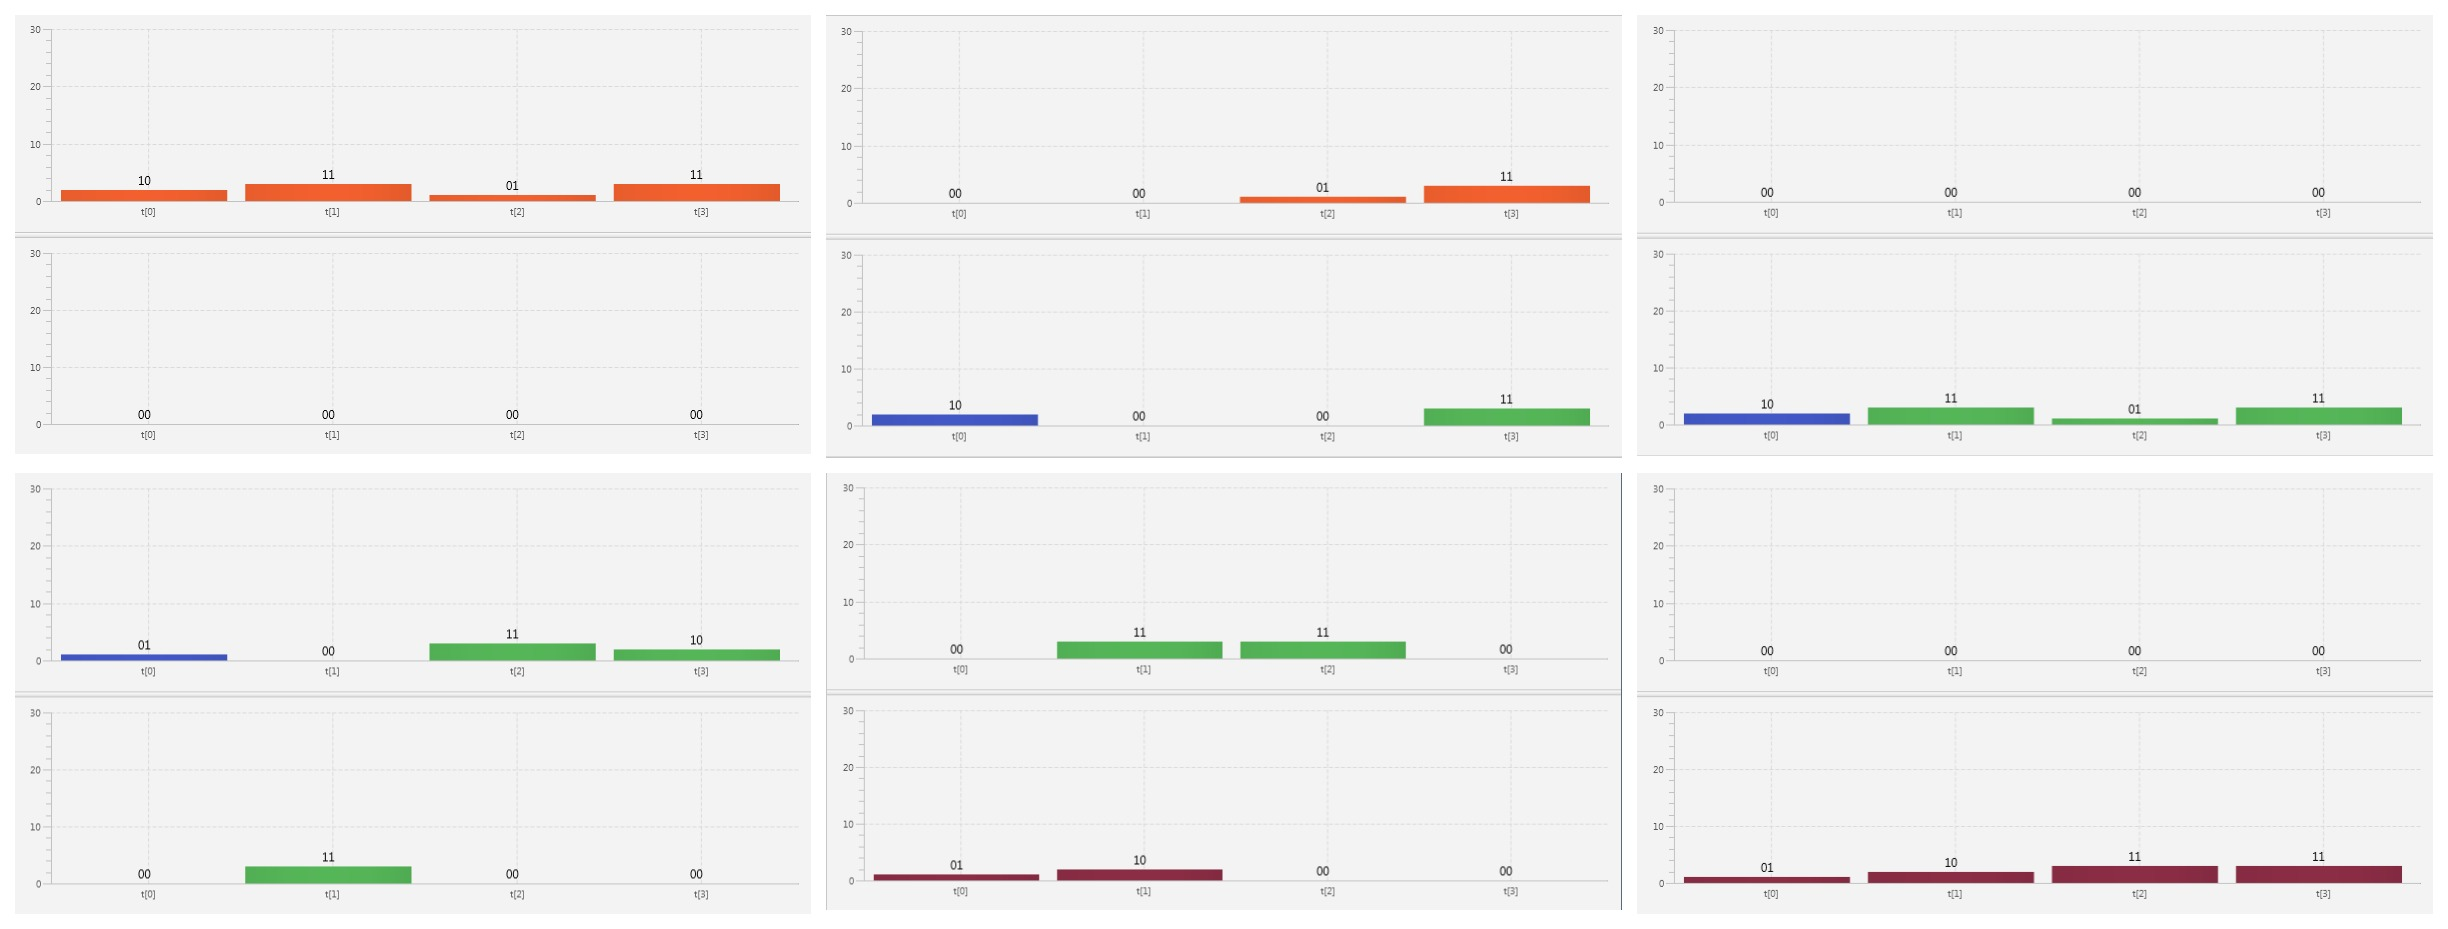
\includegraphics[width=1\textwidth]{pics/radixbackward.jpg}
 	\caption{Példa a radix "vissza" rendezésre}
 \end{figure}\par
\subsubsection{Műveletigény}
Lineáris idejű a rendezés, amennyiben $d$ jegyűek a rendezendő számok az algoritmus futási ideje:
$$T(n)=\Theta(d \cdot n) = \Theta(n)$$
\subsubsection{Jelölések az állapotjelző felületen}
Az aktuálisan vizsgált bit értékének megfelelően, amely bináris szám a 0-ás edénybe kerül \textcolor{swap}{\Huge$\bullet$}, míg amely az 1-es edénybe kerül az \textcolor{select}{\Huge$\bullet$} háttérszínt kap.

\chapter{Fejlesztői dokumentáció}

\section{Tervezés és megvalósítás}
A fejlesztés során több szempontot is figyelembe kell venni, úgy mint: műveletigény, memóriaigény, jó megjelenés, egyszerű kezelhetőség, és átlátható-, bővíthető kód készítése. Mivel ezen kritériumok közül több is csak egy másik rovására javítható, ezért a tervezés során kompromisszumokat kell kötni. Továbbá fel kell készülni arra, hogy az eredeti terven a fejlesztés során módosításokat kell végezni, mivel egy-egy probléma megoldása más megközelítést kívánhat.

\subsection{Tervezés}
A dolgozat fő célja egy olyan elsősorban hallgatóknak szánt program létrehozása, amellyel néhány rendezési algoritmus működése egy letisztult és egyszerű felhasználó felületen keresztül tanulmányozható.\par
A programnak három jól elkülönülő komponensből kell állnia:
Egy logikai(modell) részből, ami gyakorlatilag a rendszer "motorja", itt kell, hogy történjen mindenféle számítási és adattárolási művelet. Egy megjelenítési rétegből, amely a logikai rész eredményeit jeleníti meg a felhasználó számára. Végül pedig egy kontroller szintből, amely kapcsolatot teremt a logikai- és a megjelenítési réteg között. A gyakorlatban ezt a fajta tagolást nevezik Modell-Nézet-Vezérlő \emph{(MVC)} tervezési mintának.\par
Az elsődleges szempont az, hogy a felhasználó könnyedén tudja kezelni a programot, és segítségével megértse az algoritmusok működését. Így a felhasználói felület áttekinthetőségére és letisztultságára nagy hangsúlyt kell fektetni. Továbbá fontos az is, hogy a jövőben további rendezési eljárásokat is könnyedén meg lehessen jeleníteni a jelenlegiek mellett, így fontos szempont a kód egyszerű bővíthetősége.

\subsection{Megvalósítás}
Az első lépés a rendezési algoritmusok implementálása.
Ezt követhette egyszerűbb felhasználói felület létrehozása. Kezdetben elegendő, ha csak egy grafikon jelenik meg, amely reprezentálja a tömbben található számokat.\par
Két algoritmushoz szükséges a gráfos megjelenítés, így a következő lépés egy gráf implementálása.
Ezt követően a cél, hogy néhány "beégetett" elemre a rendezések lejátszhatóak legyenek, és az aktuális állapota a tömbnek szinkronban legyen a diagrammal valamint a gráffal. Később az egyes lépésekben történő összehasonlításokat/vizsgálatokat, mozgatásokat, cseréket kell különböző színekkel jelölni az állapotjelző felületeken és számon tartani ezen műveletek összegeit.\par
Ezen a ponton az módosítás történt a projekt tervein. Eredetileg egy-egy külön szálon futottak volna az algoritmusok, és a felhasználói interakció hatására ezek állapota változott volna. Azonban a \emph{JavaFX} szálkezelése jelentősen eltér az szokványos szálkezelésétől, ezért járhatóbb útnak bizonyult az, hogy kétszer kerüljenek implementálásra az algoritmusok.\par Az egyik implementációban elmentjük az interakciót követő állapotot, és ez jelenik meg a felhasználói felületen. A másik megvalósításban pedig a rendezések azonnal lezajlanak, így képet kaphatunk arról, hogy mennyi műveletre volt szükség az egyes eljárások során. Ezen utóbbi implementációk mindegyike külön szálon fut, és ahogy valamelyik befejeződik figyelmezteti a főprogramot, hogy jelenítse meg a műveletek számát. Valamint minden szálhoz egy-egy egyszerűbb egységteszteket kell készíteni.\par
Miután a program alapjai elkészültek kezdetét veheti a a felhasználói felület részletes kialakítása. Elsőként a diagram elhelyezése egy panelen, amely tartalmaz továbbá egy listát a választható algoritmusokról. Illetve egy táblázatot, melyben szerepelnek az aktuális állapot egyes tulajdonságai.\par
A programnak egy fontos szolgáltatása az, hogy a felhasználó különböző adatbeviteli mód közül választhat. A logikai réteget ki kell bővíteni ezekkel az esetekkel, továbbá a felhasználói felületen lehetőséget adni ezen módok kiválasztására.\par
Ezután az eszköztár kerül a helyére, mellyel párhuzamosan megtörténik az egyes műveletekhez tartozó eljárások implementálása.\par
Az utolsó teendő a felhasználói felületen egy rendezések összehasonlítására lehetőséget adó panel létrehozása, táblázattal, benne az algoritmusok műveletigényével. Továbbá egy diagrammal, amin megjelenik a táblázatból kiválasztott sor összehasonlításainak és mozgatásainak a száma.\par
Végül, hogy a program egyszerűen használható legyen \emph{Windows} környezetben egy telepítő fájl készítése, amellyel az előbb említett operációs rendszert használóknak nem szükséges külön \emph{Java}-t telepíteniük.


\subsection{Használt fejlesztőeszközök}
A fejlesztés \emph{Eclipse SDK 4.4} fejlesztői környezet keretei között történt. A program grafikus fejlesztői felületet ad alkalmazások készítéséhez.\par
A program elkészítése során a kódolást segítő funkció volt a kódkiegészítés, továbbá az egyik beépített projektmenedzsment eszköz(\emph{EGit}).\par
A fejlesztéshez elengedhetetlen a \emph{Java SE 8u40} vagy magasabb verziójú szoftver. Továbbá a fejlesztést nagyban elősegítette a \emph{JavaFX Scene Builder 2.0}, melynek segítségével egyszerűen megtervezhetővé váltak a grafikus felület komponensei.\par
Végül a telepítési környezet létrehozásához \emph{Ant} és \emph{InnoSetup} eszközök kerültek felhasználásra.
Az egész projekt, beleértve e dokumentumot is megtalálható, és az egyes verziók visszakövethetők a \emph{GitHub}-on: \url{https://github.com/marfoldi/SRTNGLGRTHMS}\par
A program fejlesztése során egyedüli külső függvénykönyvtár a \emph{JUnit} volt, melynek segítségével egységtesztek készültek.

\section{Használati esetek}
A következőkben a főbb használati esetek kerülnek bemutatásra. A felhasználónak tudnia kell:\par
\begin{description}
	\item[$\bullet$] rendezendő számok sorozatát megadni;
	\item[$\bullet$] algoritmust lejátszani;
	\item[$\bullet$] műveletszámokat összehasonlítani;
	\item[$\bullet$] rendezés leírását elolvasni;
	\item[$\bullet$] program névjegyét megtekinteni;
	\item[$\bullet$] programot bezárni;
	\item[$\bullet$] esetleges hibákról értesülni;
\end{description}

\section{Osztályok leírása}
A program tervezésekor az egyik alapelv volt, hogy a grafikus megjelenítés, működés szintjén minél inkább különüljön el a rendszerlogikától. A grafikus felület már csak a modell programész által számított, a vezérlő programrésznek átadott adatokat jelenítse meg. Továbbá lehetőséget biztosítson a felhasználó számára, hogy vezérelje a program rendszerlogikáját a kontroller rétegen keresztül. Ez által, hogy a rendszerlogika lényegében független a grafikus interfésztől. Így a szoftver magasabb fokú bővíthetőséget, a kód pedig jobb átláthatóságot nyer.\par
Ez az elv jól megfigyelhető a programkód struktúrájában is, alapvetően a program három fő csomagra lett bontva: A \textbf{modell} csomag, melyben a logikai osztályok találhatóak, a \textbf{view}, melyben a grafikai interfészt leíró \emph{fxml} fájlok foglalnak helyet, és végül a \textbf{controller} csomag, melyben található osztályok kapcsolatot teremtenek a logikai és a megjelenítési réteg között.

\subsection{Modell osztályok}
A modell osztályok a \textbf{modell} csomag foglalja magában. A pontosabb rendszerezést szem előtt tartva további alcsomagok kerültek létrehozásra, így jobban áttekinthető az osztályhierarchia. Összességében ebben a csomagban foglalnak helyet azon osztályok, amelyek a rendszer adattároló, rendszerező és számítási feladatait ellátják. Az alábbi táblázat ad áttekintést az előzőleg említett alcsomagokról:\par
\begin{table}[h]
		\def\arraystretch{2}
		\centering
	\begin{tabular}{|l|l|}
		\hline
		\textbf{Név}  & \textbf{Leírás}                                                                          \\ \hline
		algorithm     & A lejátszható algoritmusok implementációját tartalmazza                       \\ \hline
		algorithm.raw & Az "egyszerű" rendezést megvalósító osztályok csomagja\\ \hline
		graph         & A gráf adatszerkezet implementációja                           \\ \hline
		info         & "Az algoritmusról" felugróablakhoz tartozó adatbetöltő                         \\ \hline
	\end{tabular}
\end{table}
Elsőként a \textbf{algorithm} csomagot részletezzük, röviden az alábbi táblázat foglalja össze a benne található osztályok feladatait:

\begin{thebibliography}{widest entry}
\bibitem{Java}
\emph{Java (programming language)},
Wikipedia the free encyclopedia.
[ONLINE] [Hivatkozva: 2015.04.21]
\url{http://en.wikipedia.org/wiki/Java_(programming_language)/}
\bibitem{JavaFX}
\emph{JavaFX},
Wikipedia the free encyclopedia.
[ONLINE] [Hivatkozva: 2015.04.21]
\url{http://en.wikipedia.org/wiki/JavaFX/}
\bibitem{JUnit}
\emph{JUnit},
Wikipedia the free encyclopedia.
[ONLINE] [Hivatkozva: 2015.05.01]
\url{http://en.wikipedia.org/wiki/JUnit}
\bibitem{Demuth}
Demuth, H.:
\emph{Electronic Data Sorting},
PhD thesis, Stanford University,
1956, [184]
\bibitem{Fekete}
Dr. Fekete István:
\emph{Algoritmusok és adatszerkezetek I. jegyzet},
[ONLINE] [Hivatkozva: 2015.04.20] \url{http://people.inf.elte.hu/fekete/algoritmusok_bsc/alg_1_jegyzet/}
\bibitem{Cormen}
Thomas H. Cormen, Charles E. Leiserson,Ronald L. Rivest, Clifford Stein:
\emph{Új algoritmusok},
Scolar kiadó, 2003,
[992], 9789639193901
\bibitem{ShellWiki}
\emph{Shellsort},
Wikipedia the free encyclopedia.
[ONLINE] [Hivatkozva: 2015.04.25]
\url{http://en.wikipedia.org/wiki/Shellsort/}
\bibitem{Shell}
Donald Shell:
\emph{A high-speed sorting procedure}
Communications of the ACM, 2, 7, 1959
\bibitem{Horae}
C.A.R. Hoare:
\emph{Algorithm 64: Quicksort}
Communications of the ACM, 4, 7, 1961
\bibitem{Survey}
The Takipi Blog:
\emph{We Analyzed 30,000 GitHub Projects – Here Are The Top 100 Libraries in Java, JS and Ruby},
[ONLINE] [Hivatkozva: 2015.04.30] \url{http://blog.takipi.com/we-analyzed-30000-github-projects-here-are-the-top-100}
\url{-libraries-in-java-js-and-ruby/}
\end{thebibliography}

\end{document}
